\documentclass[11pt]{article}

\usepackage[T1]{fontenc}
\usepackage[utf8]{inputenc}
\usepackage{lmodern}
\usepackage[margin=1in]{geometry}
\usepackage{microtype}
\usepackage{amsmath,amssymb,amsthm}
\usepackage{booktabs,tabularx,multirow}
\usepackage{array}
\usepackage{graphicx}
\usepackage{xcolor}
\usepackage{siunitx}
\usepackage{enumitem}
\usepackage{listings}
\usepackage{algorithm}
\usepackage{algpseudocode}
\usepackage{tikz}
\usetikzlibrary{arrows.meta,positioning,fit,calc,shapes.geometric,backgrounds}
\usepackage{pgfplots}
\pgfplotsset{compat=1.17}
\usepackage[numbers,sort&compress]{natbib}
\usepackage[colorlinks=true,linkcolor=blue!50!black,citecolor=green!35!black,urlcolor=blue!60!black]{hyperref}
\usepackage[capitalise,noabbrev]{cleveref}

% Notation from the AVO paper
\newcommand{\Pt}{\mathcal{P}_t}
\newcommand{\Pop}{\mathcal{P}}
\newcommand{\K}{\mathcal{K}}
\newcommand{\f}{\mathbf{f}}
\newcommand{\Vary}{\mathrm{Vary}}
\newcommand{\Agent}{\mathrm{Agent}}
\newcommand{\Generate}{\mathrm{Generate}}
\newcommand{\Sample}{\mathrm{Sample}}
\newcommand{\Update}{\mathrm{Update}}
\newcommand{\pass}{\mathrm{pass}}
\newcommand{\cfgs}{\mathcal{C}}

% Code and command names
\newcommand{\cmd}[1]{\texttt{#1}}
\newcommand{\file}[1]{\texttt{#1}}
\newcommand{\avo}[1]{\texttt{avo~#1}}

% Theorem-like environments
\theoremstyle{definition}
\newtheorem{definition}{Definition}
\newtheorem{proposition}{Proposition}
\theoremstyle{remark}
\newtheorem*{remark}{Remark}

% Listings
\definecolor{codebg}{gray}{0.96}
\lstset{
  basicstyle=\ttfamily\footnotesize,
  backgroundcolor=\color{codebg},
  frame=single, framerule=0pt,
  columns=fullflexible, keepspaces=true,
  breaklines=true, breakatwhitespace=true,
  showstringspaces=false,
  xleftmargin=4pt, xrightmargin=4pt,
  aboveskip=6pt, belowskip=6pt
}

% TikZ styles
\tikzset{
  box/.style={draw, rounded corners=3pt, align=center, minimum height=1.0cm,
              minimum width=2.6cm, font=\small, fill=white},
  hl/.style={box, fill=gray!15, thick},
  store/.style={draw, rounded corners=3pt, align=left, font=\footnotesize, fill=blue!4},
  arr/.style={-{Stealth[length=2.2mm]}, thick},
  darr/.style={-{Stealth[length=2.2mm]}, thick, dashed},
  lbl/.style={font=\footnotesize, align=center},
}


\title{An implementation of NVIDIA's Agentic Variation Operators (AVO)\\
for Autonomous Evolutionary Search}
\author{Marcos Cannabrava\\
\small\url{https://github.com/marcoscannabrava/avocode}}
\date{October 2026}

\begin{document}
\maketitle

\begin{abstract}
Agentic Variation Operators (AVO) replace the fixed mutation and crossover steps of evolutionary
search with an autonomous coding agent: $\Vary(\Pt) = \Agent(\Pt, \K, \f)$. NVIDIA used AVO to
evolve attention kernels on B200 GPUs for seven days, and the result beat cuDNN and
FlashAttention-4. The paper did not release its harness, its agent or its supervisor.

This article describes \emph{avocode}, an open, agent-agnostic implementation of the AVO harness.
avocode maps each formal object of AVO to a concrete artifact in a git repository. The scoring
function $\f$ is an executable that prints one JSON line. The lineage $\Pt$ is a chain of git commits
with score trailers. The knowledge base $\K$ is a hybrid-search index over documents \emph{and} over
the lineage itself. The agent is any of three coding agents (pi, Claude Code or Codex), driven by
five portable skill files. We make precise what the paper leaves open. The commit rule is weak
Pareto dominance over a score vector, with strict gain on at least one configuration and a
relative noise floor. The supervisor is a deterministic detector of two signals, \emph{stall} and
\emph{thrash}, that emits a directive citing prior versions, recorded dead ends and unread
documents. A fan-out operator runs $N$ probes in disposable git worktrees as a bounded first step
toward the population search that the paper leaves as future work.

On a fuzzy string search benchmark, two runs of the loop with Claude Code (65 minutes in total)
committed seven versions and cut the median search time from \SI{1810}{ms} to \SI{0.231}{ms}, a
$7837\times$ speedup, with no regression committed. One of the seven steps, a pigeonhole partition
index, is absent from the hand-written reference solutions. We also report what this evidence does
not show. The supervisor never fired in a real run, all results come from one benchmark and one
agent, and the integrity of $\f$ rests partly on convention rather than enforcement.
\end{abstract}

\section{Introduction}
\label{sec:intro}

Evolutionary search improves a solution by repeating two steps. A \emph{variation} operator makes
new candidates from old ones, and a \emph{selection} step keeps the better ones
\citep{back1997handbook}. For decades the variation operator was hand-designed: bit flips,
subtree swaps and crossover \citep{oneill2010openissues}. Large language models (LLMs) changed this. In
ELM \citep{lehman2022elm}, FunSearch \citep{romeraparedes2024funsearch}, EvoPrompting
\citep{chen2023evoprompting} and AlphaEvolve \citep{novikov2025alphaevolve}, an LLM writes the new
candidate. But a fixed framework still samples the parents, runs the evaluation and manages the
population. The LLM fills one slot in a pipeline:
\begin{equation}
  \Vary(\Pt) = \Generate\big(\Sample(\Pt)\big).
  \label{eq:intro-generate}
\end{equation}

The AVO paper \citep{chen2026avo} argues that this slot is too small. An LLM confined to
$\Generate$ ``produces a single output per invocation, with no ability to proactively consult
reference materials, test its changes, interpret feedback, or revise its approach before committing
a candidate'' \citep[\S1]{chen2026avo}. AVO gives the whole variation step to an autonomous coding
agent:
\begin{equation}
  \Vary(\Pt) = \Agent(\Pt, \K, \f),
  \label{eq:intro-agent}
\end{equation}
where $\Pt$ is the lineage of solutions and their scores, $\K$ is a domain knowledge base and $\f$
is the scoring function. The agent decides what to read, what to edit and when to test. NVIDIA ran
this operator for seven days on multi-head attention for Blackwell B200 GPUs. It committed 40
versions and reached up to \SI{1668}{TFLOPS}, which is up to 3.5\% faster than cuDNN and up to
10.5\% faster than FlashAttention-4 on the tested configurations.

The paper's result is about kernels. Its \emph{harness} is not. Equation~\eqref{eq:intro-agent}
needs only four things: a way to measure a candidate, a record of the versions that survived, a
place to look things up, and an agent. None of them is specific to GPUs. But the paper releases no
code, names no model and gives no supervisor thresholds. It leaves the acceptance rule for a
vector score as the phrase ``matches or improves''. A reader who wants to apply AVO to a different
problem has to rebuild the harness from the prose.

This article describes such a rebuild. \emph{avocode} is a command-line tool (\cmd{avo}) and a set
of agent skills that turn any git repository with a measurable score into an AVO loop. Its thesis
is that the harness generalizes past attention kernels to any repository with a strict, cheap
scorer. The design follows one rule throughout: the agent proposes, and the measurement decides.

\paragraph{Contributions.}
\begin{enumerate}[leftmargin=*,itemsep=2pt]
  \item \textbf{A concrete mapping of AVO to a repository} (\cref{sec:overview}). $\f$ becomes an
    executable with a one-line JSON contract, $\Pt$ becomes git commits with score trailers, and
    $\K$ becomes a hybrid-search index whose corpus includes the lineage itself.
  \item \textbf{A precise commit rule} (\cref{sec:lineage}). We define acceptance as weak Pareto
    dominance over the score vector with strict gain on at least one configuration and a
    symmetric relative noise floor. We state the invariants this rule gives and the ways it
    resists gaming.
  \item \textbf{An external, deterministic supervisor} (\cref{sec:supervise}). It detects two
    signals, stall and thrash, and emits a directive that \emph{cites} prior versions, recorded
    dead ends and documents in $\K$ that no version has used.
  \item \textbf{Agent-agnostic delivery} (\cref{sec:adapters}). The same five skill files drive
    pi, Claude Code and Codex. Every capability is reachable from a shell.
  \item \textbf{A bounded fan-out operator} (\cref{sec:fan}). \avo{fan} runs $N$ probes in
    disposable git worktrees on a small model. It is a first, local step toward the population
    search that the paper defers.
  \item \textbf{An empirical case study and an honest list of limits} (\cref{sec:eval,sec:limits}).
    Two runs on a fuzzy search benchmark reach a $7837\times$ speedup with no committed
    regression. We also show where the evidence is thin.
\end{enumerate}

\paragraph{Outline.} \Cref{sec:background} places AVO among related work. \Cref{sec:avo}
summarizes the AVO paper. \Cref{sec:overview,sec:score,sec:lineage,sec:orchestration} describe
avocode, from the system view down to the commit rule and the loop. \Cref{sec:eval} reports
results. \Cref{sec:discussion} compares avocode with the paper, and \cref{sec:limits} lists
limitations and future work.

\section{Background and related work}
\label{sec:background}

\subsection{Classical evolutionary computation}

Genetic algorithms \citep{holland1992adaptation} and genetic programming \citep{koza1992gp} keep a
population, vary it with blind syntactic operators, and select by fitness. Genetic programming is
the direct ancestor of ``evolve code against an executable fitness function''. Its long-standing
problems include operator locality, where a small syntactic change causes a large semantic change,
and poor scaling to large programs \citep{oneill2010openissues}. The AVO paper cites this survey to
motivate operators that understand code.

The closest classical model of avocode is the $(1+1)$ evolutionary algorithm
\citep{back1997handbook,droste2002oneplusone}. It keeps one parent, mutates it, and keeps the child
if it is at least as good. avocode differs in two ways. It accepts by dominance over a score vector
rather than by a scalar $\geq$, and it refuses ties, so it allows no neutral drift. With \avo{fan},
the scheme becomes $(1+\lambda)$: $\lambda$ probes run in parallel, and at most one is promoted. A
single elitist lineage is a hill climber, and its known failure is stagnation at a local optimum
\citep{russell2020aima}. Novelty search \citep{lehman2011novelty} and quality-diversity archives
such as MAP-Elites \citep{mouret2015mapelites} answer this by keeping diverse stepping stones.
AVO and avocode drop the archive on purpose and rely on the agent, which reads the whole lineage,
to supply diversity. \Cref{sec:limits} returns to this cost.

\subsection{LLMs as variation operators}

ELM \citep{lehman2022elm} first used a code LLM as the mutation operator inside MAP-Elites.
Language model crossover \citep{meyerson2024lmx} puts several parents in one prompt. EvoPrompting
\citep{chen2023evoprompting}, EvoPrompt \citep{guo2023evoprompt} and Promptbreeder
\citep{fernando2023promptbreeder} evolve architectures and prompts in the same way. OPRO
\citep{yang2024opro} is the simplest ``lineage in context'' optimizer: past solutions and their
scores go into the prompt. FunSearch \citep{romeraparedes2024funsearch} paired a code LLM with an
evaluator and an island-based program database, and found new cap-set constructions. AlphaEvolve
\citep{novikov2025alphaevolve} scaled this to whole files, an LLM ensemble and asynchronous
evaluators, with results in matrix multiplication, scheduling and kernels
\citep{georgiev2025mathexploration}. ReEvo \citep{ye2024reevo} adds a reflection stage, and
LoongFlow \citep{wan2025loongflow} replaces random mutation with a plan--execute--summarize cycle.

Open re-implementations exist. OpenEvolve \citep{sharma2025openevolve} rebuilds AlphaEvolve's
pipeline. ShinkaEvolve \citep{lange2025shinkaevolve} adds novelty rejection and a bandit over
models for sample efficiency, and CodeEvolve \citep{assumpcao2025codeevolve} uses island search
over a CVT-MAP-Elites archive. These all implement the fixed $\Generate \circ \Sample$ pipeline that
AVO removes. The avocode design notes reject them as a base for this reason. Another line changes
the operator's weights rather than its context, through test-time reinforcement learning
\citep{yuksekgonul2026ttdiscover,yan2026pacevolve}. avocode trains nothing; it only shapes the
context through the lineage, memory and knowledge.

\subsection{Coding agents and autonomous research loops}

AVO depends on agents that can work at repository scale. ReAct \citep{yao2023react} interleaves
reasoning and tool use. SWE-bench \citep{jimenez2024swebench} measures real issue resolution, and
SWE-agent \citep{yang2024sweagent} shows that the agent--computer interface matters: a few
well-designed commands raise scores a lot. avocode is an interface of this kind for evolution. It
gives the agent a few commands with JSON output, and skills that say when to use each one. The
operators it drives are pi \citep{zechner2025pi}, Claude Code \citep{anthropic2025claudecode} and
Codex \citep{openai2025codexcli}; OpenHands \citep{wang2025openhands} could be added with one
template.

Reflexion \citep{shinn2023reflexion} stores verbal reflections after a failure, and Voyager
\citep{wang2023voyager} keeps a library of executable skills. avocode makes both explicit and
durable: dead ends and insights go to memory that a new session reads, and skills are files in the
repository. AIDE \citep{jiang2025aide} searches a tree of scripts. The AI Scientist
\citep{lu2024aiscientist,yamada2025aiscientistv2} automates a full research pipeline. The Darwin
G\"odel Machine \citep{zhang2025dgm} evolves the agent itself, as do STOP, G\"odel Agent and ADAS
\citep{zelikman2023stop,yin2024godelagent,hu2025adas}. These systems improve the operator; AVO and
avocode improve a target with a fixed operator.

The closest relatives of avocode appeared in 2026. Karpathy's \emph{autoresearch}
\citep{karpathy2026autoresearch} is a minimal loop: an agent edits one training script, runs a
five-minute job, and keeps the change only if validation loss improves. avocode generalizes it with
a scorer contract, a score vector with a noise floor, recorded refusals, searchable memory, parallel
probes and a supervisor. Bilevel Autoresearch \citep{qu2026bilevel} shows that improving the harness
can matter as much as the model. Agora \citep{zhang2026agora} also uses git as the store of results,
as a directed acyclic graph shared by many workers. SEDIMA \citep{abaskohi2026sedima} adds a memory of
insights to evolutionary agents because memoryless search ``rediscovers the same improvements and
re-encounters the same dead ends''. Chun et al.\ \citep{chun2026wastedcompute} list the failure
modes of such agents: they fix the same bugs again and again and do not explore. avocode's dead-end
memory, thrash detector and fan-out target exactly these modes.

\subsection{LLMs for performance engineering}

The FlashAttention series \citep{dao2022flashattention,dao2023flashattention2,shah2024flashattention3,zadouri2026flashattention4}
and cuDNN \citep{chetlur2014cudnn} are AVO's baselines. KernelBench
\citep{ouyang2025kernelbench} measures whether LLM kernels are both correct and fast, which has the
same shape as avocode's $\f$: a correctness gate, then a metric. Kevin \citep{baronio2025kevin},
CUDA-L1 \citep{li2025cudal1} and CUDA Agent \citep{dai2026cudaagent} train the refinement loop into
the model; AVO and avocode put it into the harness. SOL-ExecBench \citep{lin2026solexecbench}
scores against speed-of-light bounds, which a scorer could report as an absolute scale.

\subsection{Evaluation integrity}

An optimizer under strong pressure games its proxy
\citep{manheim2018goodhart,amodei2016concrete,krakovna2020specgaming}. Evolutionary search has
exploited bugs in fitness functions for decades \citep{lehman2020surprising}. With agents, the
problem is faster and deliberate. METR reports frontier models that read the grader's answer or
patch the timer \citep{metr2025rewardhacking}; in one case a model took the reference output from
the call stack and disabled CUDA synchronization to fake a fast kernel. Sakana's AI CUDA Engineer
\citep{lange2025aicudaengineer} withdrew speedups that came from an evaluation exploit, and
robust-kbench \citep{lange2025robustkbench} closes such loopholes. ImpossibleBench
\citep{zhong2025impossiblebench} measures how often agents exploit tests. The AVO paper does not
discuss this threat in detail. avocode treats it as a first-class design concern
(\cref{sec:gaming}).

\Cref{tab:landscape} places avocode among these systems.

\begin{table}[t]
\centering\small
\caption{Where avocode sits. ``Pipeline'' denotes FunSearch, AlphaEvolve, OpenEvolve and
ShinkaEvolve.}
\label{tab:landscape}
\begin{tabularx}{\linewidth}{@{}l X X X@{}}
\toprule
Axis & Pipeline systems & AVO & avocode \\
\midrule
Operator & one LLM call in a fixed pipeline & one internal agent loop & any coding agent (pi, Claude Code, Codex) \\
Selection & population, islands, MAP-Elites & single lineage, ``matches or improves'' & single lineage; vector dominance with a noise floor \\
Diversity & archive, islands & agent reads the lineage & agent, \avo{fan} probes, supervisor \\
Memory & program database & conversation history & git lineage, searchable $\K$, dead-end memory \\
Integrity & sandboxed evaluator & not discussed & re-score at commit, no measuring less, hash gates, external audit \\
Release & open (OpenEvolve, ShinkaEvolve) & none & open source \\
\bottomrule
\end{tabularx}
\end{table}

\section{AVO in brief}
\label{sec:avo}

This section summarizes the AVO paper \citep{chen2026avo} (arXiv v1, March 2026). We keep its
notation. Where the paper is silent, we say so, because those gaps are where an implementation must
make choices.

\subsection{Formulation}

Generic evolutionary search keeps a population $\Pop = \{(x_i, \f(x_i))\}$ of solutions and their
scores, and repeats
\begin{equation}
  \Pop_{t+1} = \Update\big(\Pt, (x_{t+1}, \f(x_{t+1}))\big), \qquad x_{t+1} = \Vary(\Pt).
  \label{eq:evo}
\end{equation}
Prior LLM methods split $\Vary$ into $\Generate \circ \Sample$ (\cref{eq:intro-generate}). The paper
notes that ``the LLM only participates in Generate: the sampling strategy, evaluation protocol,
population management, and the order of operations are all determined by the framework''
\citep[\S2.1]{chen2026avo}. AVO replaces the whole operator with one agent run
(\cref{eq:intro-agent}). The agent ``subsumes Sample, Generate, and evaluation into a single
autonomous loop''.

The objects are:
\begin{itemize}[leftmargin=*,itemsep=1pt]
  \item $\Pt = \{(x_1, \f(x_1)), \ldots, (x_t, \f(x_t))\}$, ``the full lineage of solutions and their
    scores''. In the experiments, each $x_i$ is a CUDA kernel with inline PTX.
  \item $\f(x_i) = (f_1(x_i), \ldots, f_n(x_i))$, a vector with one component per test
    configuration. A candidate that fails the correctness check gets $f_j(x_i) = 0$ for all $j$,
    ``regardless of throughput''.
  \item $\K$, a knowledge base: CUDA guides, the PTX ISA, Blackwell specifications, and existing
    kernels including the FlashAttention-4 source.
\end{itemize}

\subsection{One variation step}

A step that produces $x_{t+1}$ is an autonomous agent loop with ``numerous internal actions''. The
agent often reads several prior versions in $\Pt$, compares their profiles, and consults $\K$ before
it edits. It then calls $\f$. If the candidate fails or does not improve, the agent diagnoses and
revises. The paper calls this the \emph{edit--evaluate--diagnose} cycle. The rule for keeping a
result is stated once:
\begin{quote}\small
``we persist a new committed version only when it passes correctness checks and matches or improves
the benchmark score relative to the best committed version so far; unsuccessful intermediate
attempts remain part of the agent's internal search trajectory but are not added to the committed
lineage.'' \citep[\S3.2]{chen2026avo}
\end{quote}
Read literally, this is an elitist, monotone update: $\Pop_{t+1} = \Pt \cup \{(x', \f(x'))\}$ if
$x'$ is correct and scores at least as well as the best, and $\Pop_{t+1} = \Pt$ otherwise. Nothing is
pruned. The paper does not say how ``matches or improves'' applies to a \emph{vector}, or what
tolerance counts as a match. Its trajectory plots use the geometric mean across configurations,
which suggests a scalar reduction, but the text does not commit to one.

\subsection{Continuous evolution and the supervisor}

The paper runs AVO as a single lineage from a seed $x_0$, ``leaving population-level branching and
archive management to future extensions'' \citep[\S3.3]{chen2026avo}. Each committed version is a
git commit with its score. Two failure modes appear in long runs: the agent can \emph{stall} when it
exhausts a line of exploration, or it can enter ``unproductive cycles of edits that repeatedly fail
to improve scores''. A self-supervision mechanism detects both. When triggered, it ``reviews the
overall evolutionary trajectory and steers the search toward several candidate optimization
directions''. Figure~2 of the paper draws this as a separate \emph{AVO Supervisor Agent}. The paper
gives no thresholds, no trigger counts, and no mechanism for how the directions reach the main
agent.

The agent itself is ``an internally-developed general-purpose coding agent powered by frontier
LLMs'' with code editing, shell, file navigation and documentation retrieval. Its memory is its
conversation history. The models are not named, and no token or cost figures are given.

\subsection{Reported results}

\Cref{tab:avo-results} summarizes the results on B200 (forward prefill, head dimension 128, BF16,
sequence lengths 4K--32K at a fixed 32K total tokens). The seven-day run produced 40 versions and
explored ``over 500 candidate optimization directions''. Gains came in discrete jumps, for example
branchless accumulator rescaling ($+8.1\%$ non-causal at v20) and register rebalancing across warp
groups ($+2.1\%$ at v33). The paper uses these to argue that the agent performs ``genuine
hardware-level reasoning rather than superficial code transformations''. Adapting the final kernel
to grouped-query attention (GQA) took 30 more minutes of autonomous work.

\begin{table}[t]
\centering\small
\caption{Headline results of the AVO paper \citep[\S4]{chen2026avo}. Ranges are over the four
sequence lengths. TFLOPS values are the paper's bar labels.}
\label{tab:avo-results}
\begin{tabular}{@{}lccc@{}}
\toprule
Workload & Peak AVO TFLOPS & vs.\ cuDNN & vs.\ FlashAttention-4 \\
\midrule
MHA, causal      & 1637 & $+0.4\%$ to $+3.5\%$ & $+5.0\%$ to $+10.5\%$ \\
MHA, non-causal  & 1668 & $+1.8\%$ to $+2.4\%$ (16K, 32K) & within noise at 4K, 8K \\
GQA, causal      & 1647 & up to $+7.0\%$ & up to $+9.3\%$ \\
GQA, non-causal  & 1679 & up to $+6.0\%$ & up to $+4.5\%$ \\
\midrule
\multicolumn{4}{@{}l}{Run: 7 days, 40 committed versions, $>$500 directions explored, 1 lineage.}\\
\bottomrule
\end{tabular}
\end{table}

\subsection{What the paper leaves open}
\label{sec:avo-open}

For an implementer, the important gaps are:
\begin{enumerate}[leftmargin=*,itemsep=1pt]
  \item \textbf{No code or harness.} No repository, prompts, or agent configuration.
  \item \textbf{An underspecified acceptance rule.} ``Matches or improves'' on a vector, with no
    noise band, although the authors measured each benchmark 10 times for mean and deviation.
  \item \textbf{An unspecified supervisor.} No detection rule, threshold, or delivery mechanism.
  \item \textbf{Trajectory is lost.} Failed attempts live only in the agent's context, so a new
    session cannot learn from them.
  \item \textbf{No population.} Branching and archives are future work.
  \item \textbf{No ablations of the harness.} Neither $\K$ nor the supervisor is ablated, and AVO is
    not compared with a $\Generate \circ \Sample$ baseline on the same budget.
\end{enumerate}
avocode gives a concrete answer to items 1--4 and a partial answer to item 5. It does not address
item 6. \Cref{sec:discussion} returns to each.

\section{System overview}
\label{sec:overview}

avocode extracts the AVO harness and makes it independent of the agent and of the domain.
\Cref{tab:mapping} gives the mapping from the paper's objects to artifacts in a repository.
\Cref{fig:loop} shows the loop.

\begin{table}[t]
\centering\small
\caption{How avocode implements each object of AVO.}
\label{tab:mapping}
\begin{tabularx}{\linewidth}{@{}l l X l@{}}
\toprule
Symbol & Meaning & avocode artifact & Module \\
\midrule
$\f$ & scoring function & executable \file{.avo/score} printing one JSON line & \file{score.ts} \\
$\succ$ & order on $\f$ & vector comparator, noise floor, reduction & \file{compare.ts} \\
$\Pt$ & lineage & git commits with \cmd{Avo-Version}/\cmd{Avo-Score} trailers, \cmd{git notes}, \file{lineage/vNNN.md} & \file{lineage.ts} \\
$\K$ & knowledge base & \file{knowledge/} $+$ \file{lineage/}, hybrid search; web ingest with provenance & \file{knowledge.ts} \\
-- & agent memory & beads issue graph, or \file{lineage/memory.jsonl} & \file{mem.ts} \\
$\Agent$ & variation operator & pi, Claude Code or Codex, driven by five skills & \file{agents.ts} \\
-- & supervisor & stall/thrash detector with a citing directive & \file{supervise.ts} \\
-- & trajectory & \file{.avo/attempts.jsonl}, \file{.avo/runs/}, \file{.avo/worktrees/} (never committed) & \file{score.ts} \\
\bottomrule
\end{tabularx}
\end{table}

\begin{figure}[t]
\centering
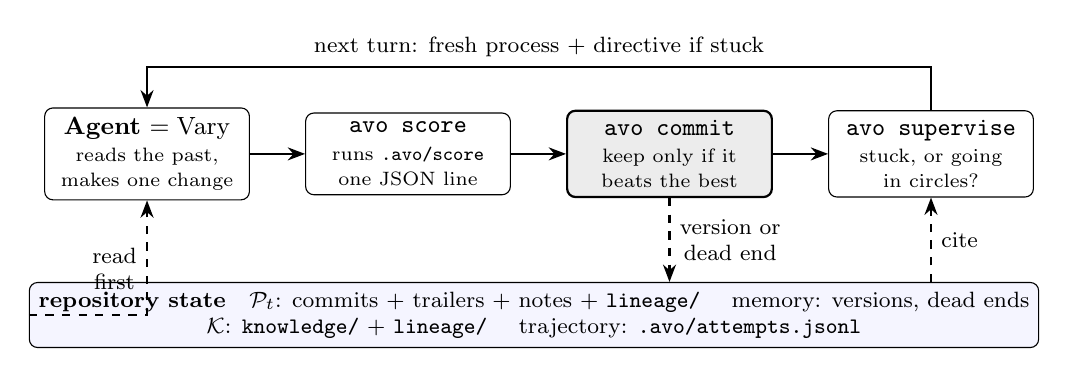
\begin{tikzpicture}[node distance=0.55cm and 0.7cm]
  \node[box] (agent) {\textbf{Agent} $=\Vary$\\[-1pt]\scriptsize reads the past,\\[-2pt]\scriptsize makes one change};
  \node[box, right=of agent] (score) {\textbf{\cmd{avo score}}\\[-1pt]\scriptsize runs \file{.avo/score}\\[-2pt]\scriptsize one JSON line};
  \node[hl, right=of score] (commit) {\textbf{\cmd{avo commit}}\\[-1pt]\scriptsize keep only if it\\[-2pt]\scriptsize beats the best};
  \node[box, right=of commit] (sup) {\textbf{\cmd{avo supervise}}\\[-1pt]\scriptsize stuck, or going\\[-2pt]\scriptsize in circles?};
  \node[store, below=1.1cm of score, xshift=1.6cm, minimum width=8.4cm, align=center] (st)
    {\textbf{repository state}\quad $\Pt$: commits $+$ trailers $+$ notes $+$ \file{lineage/}
     \quad memory: versions, dead ends\\ $\K$: \file{knowledge/} $+$ \file{lineage/}
     \quad trajectory: \file{.avo/attempts.jsonl}};
  \draw[arr] (agent) -- (score);
  \draw[arr] (score) -- (commit);
  \draw[arr] (commit) -- (sup);
  \draw[arr] (sup.north) -- ++(0,0.55) -| node[pos=0.25, above, lbl]
    {next turn: fresh process $+$ directive if stuck} (agent.north);
  \draw[darr] (st.west) -| node[pos=0.7, left, lbl] {read\\first} (agent.south);
  \draw[darr] (commit.south) -- node[right, lbl] {version or\\dead end} (commit.south |- st.north);
  \draw[darr] (st.north -| sup.south) -- node[right, lbl] {cite} (sup.south);
\end{tikzpicture}
\caption{The avocode loop. The agent proposes; the score and the commit rule decide. Every
outcome, kept or refused, is written to the repository that the next turn reads.}
\label{fig:loop}
\end{figure}

\subsection{Three layers}

avocode has three layers, and only the first is required.
\begin{description}[leftmargin=*,itemsep=2pt,font=\normalfont\bfseries]
  \item[CLI.] \file{bin/avo} is a bash shim that runs \file{src/main.ts} through \cmd{tsx}. There is
    no build step. The CLI is the only interface that must exist. An invariant of the design is
    that every capability is reachable from \cmd{bash} before it gets any other binding.
  \item[Skills.] Five Markdown files in \file{.agents/skills/} follow the Agent Skills format
    \citep{agentskills2025spec}. They teach an agent the loop: \cmd{avo-vary} (one variation step),
    \cmd{avo-score} (the $\f$ contract), \cmd{avo-lineage} (reading $\Pt$), \cmd{avo-knowledge}
    ($\K$) and \cmd{avo-fanout} (parallel probes). The project calls the skills ``the product'':
    the CLI enforces, and the skills teach.
  \item[Bindings.] Native tools and an in-session supervisor for the pi agent
    (\cref{sec:adapters}). These add convenience, never capability.
\end{description}

\subsection{One file, one contract}

Each source file owns one contract (\cref{tab:modules}). The pi extension imports the same files
as the CLI, so the commit rule, the detector and the recursion guards each exist once. Every
external effect goes through an injectable seam: an \cmd{Io} sink for output, a \cmd{Runner} for
processes and a \cmd{Fetcher} for the network. This is why the 441 unit tests run without a
terminal, a scorer, git or a network.

\begin{table}[t]
\centering\small
\caption{Source modules of avocode (TypeScript, about 9{,}100 lines in \file{src/}).}
\label{tab:modules}
\begin{tabularx}{\linewidth}{@{}l X r@{}}
\toprule
File & Owns & Lines \\
\midrule
\file{cli.ts} & subcommand dispatch, flags, exit codes & 162 \\
\file{score.ts} & $\f$: run \file{.avo/score}, validate, normalize into an attempt & 644 \\
\file{config.ts} & \file{.avo/config.json}: reduction, noise floor, configs, thresholds & 172 \\
\file{compare.ts} & the commit rule's comparator over the score vector & 235 \\
\file{lineage.ts} & $\Pt$: \avo{commit}, \avo{lineage}, \avo{best} & 805 \\
\file{mem.ts} & memory: beads with a JSONL fallback & 447 \\
\file{knowledge.ts} & $\K$: qmd collections, local fallback, ingest with provenance & 985 \\
\file{websearch.ts} & $\K$ from the web: three backends behind one seam & 324 \\
\file{agents.ts} & headless agent templates; one turn as \cmd{fan} and \cmd{run} see it & 436 \\
\file{fan.ts} & \avo{fan}: worktrees, probes, guards, promote, resume & 1065 \\
\file{supervise.ts} & \avo{supervise}: stall/thrash detector and directive & 550 \\
\file{run.ts} & \avo{run}: the continuous loop and its manifest & 823 \\
\file{init.ts}, \file{install.ts}, \file{doctor.ts}, \file{skills.ts} & scaffolding, agent wiring, dependency checks, skill validation & 927 \\
\bottomrule
\end{tabularx}
\end{table}

\subsection{Design invariants}
\label{sec:invariants}

The design document lists nine invariants. They explain most choices in the rest of the article.
\begin{enumerate}[leftmargin=*,itemsep=1pt]
  \item \avo{commit} is the only writer of the committed lineage.
  \item A failing $\f$ never yields a commit.
  \item Every subcommand supports \cmd{--json}.
  \item Degrade, never crash: each optional tool has a named fallback and one warning.
  \item Idempotent by construction (\cmd{init}, \cmd{install}, \cmd{commit}).
  \item Never leak secrets: report the presence of a key, never its value.
  \item Worktrees are disposable; the main branch is not.
  \item CLI first: a capability is reachable from \cmd{bash} before any binding.
  \item The skills are the product.
\end{enumerate}

\section{The scoring function \texorpdfstring{$\f$}{f}}
\label{sec:score}

In AVO, $\f$ checks correctness against a reference and measures throughput per configuration. In
avocode, $\f$ is any executable at \file{.avo/score}, run from the repository root. This keeps the
harness domain-free: a benchmark, a test suite, or a game simulator can all be a scorer.

\subsection{The contract}

The scorer has three call forms:
\begin{lstlisting}
.avo/score                   # score everything; print one JSON line
.avo/score --configs         # optional: list config names, one per line
.avo/score --config <name>   # score one config; print one JSON line
\end{lstlisting}
It must print one JSON object and should always exit 0. A typical line is:
\begin{lstlisting}
{"ok":true,"correct":true,"primary":0.231,"unit":"ms","higher_is_better":false,
 "scores":{"small":0.158,"large":0.304}}
\end{lstlisting}
The fields \cmd{ok}, \cmd{correct}, \cmd{primary} (a number or \cmd{null}), \cmd{unit} and
\cmd{higher\_is\_better} are required. The fields \cmd{scores} (the vector), \cmd{log} and
\cmd{duration\_s} are optional. Unknown keys are allowed, but each one produces a warning, so a typo
such as \cmd{higherIsBetter} reports both a missing and an unknown field.

The two booleans have different meanings. \cmd{ok} says that \emph{the scorer} worked; it is not a
verdict on the candidate. \cmd{correct} is \emph{the gate}. avocode defines
\begin{equation}
  \pass(x) = \mathrm{ok}(x) \wedge \mathrm{correct}(x).
\end{equation}
If $\neg\pass(x)$, avocode sets \cmd{primary} to \cmd{null}, whatever the scorer measured. This
generalizes the paper's ``assign zero score''. Zero is the \emph{best} possible value of a
lower-is-better metric such as latency, so it cannot mean failure in a domain-free harness.

\subsection{Harness errors and results}

avocode separates a candidate that fails from a scorer that fails. A spawn failure, a timeout, or
output that does not parse is a \emph{harness error} (exit 2). A valid JSON line with
$\neg\pass$ is a \emph{result} (exit 1). Only results teach anything about the candidate, so only
results feed memory and the supervisor (\cref{sec:refusal}). The parser scans standard output
backwards for the last line that parses as a JSON object, so build noise before the payload is
harmless.

Each scorer run is spawned as the leader of its own process group. On timeout avocode sends
\cmd{SIGKILL} to the whole group, which also kills benchmark processes that the scorer started.
Output is capped at 200{,}000 characters per stream as a 150{,}000-character head plus a rolling
50{,}000-character tail. The tail exists because the payload comes \emph{last}. An earlier
head-only cap dropped the final event of agent logs and recorded 44 input tokens for a run that sent
985{,}039 (\cref{sec:eval-cost}).

\subsection{Configurations and the score vector}

A scorer may report a vector in \cmd{scores}, one entry per configuration, which matches the
paper's $\f = (f_1, \ldots, f_n)$. With \cmd{--parallel}, avocode asks the scorer for its config
names and runs \cmd{.avo/score --config <name>} for each, with at most
$\max(1, \min(8, \mathit{cpus} - 2))$ in parallel. One failing config fails the whole attempt.
\cmd{primary} is the arithmetic mean of the per-config primaries; it is a headline only. The commit
rule uses the vector (\cref{sec:commit-rule}).

\subsection{The attempt log}

Every scorer run appends one record to \file{.avo/attempts.jsonl}, including the git
\cmd{HEAD} and a dirty flag. This is the \emph{trajectory}: the attempts that the paper leaves
inside the agent's context. In avocode it is a file on disk. It is never committed, but the
supervisor reads it (\cref{sec:supervise}).

\subsection{Templates and scorer design}

\avo{score --init} copies one of three templates: \cmd{hyperfine} (mean seconds per config, lower is
better, \cmd{correct} = a test command passes), \cmd{pytest} and \cmd{vitest} (pass rate, higher is
better). The documentation gives four rules for writing a scorer, and they matter more than any
code in the harness:
\begin{enumerate}[leftmargin=*,itemsep=1pt]
  \item Make \cmd{correct} strict and cheap. It is the only thing that rejects a fast wrong answer.
  \item Make the benchmark deterministic, or set a noise floor (\cref{sec:commit-rule}).
  \item Keep it fast. A one-hour scorer allows 24 attempts a day.
  \item Measure what you want improved, because that is what the agent will optimize.
\end{enumerate}
\Cref{sec:eval-bench} shows two scorers built on these rules, with hash gates over protected files
and a full-scale differential check against an independent reference.

\section{The lineage \texorpdfstring{$\Pt$}{P\_t}, memory and knowledge \texorpdfstring{$\K$}{K}}
\label{sec:lineage}

\subsection{The commit rule}
\label{sec:commit-rule}

The commit rule is the selection step of the evolutionary search. In avocode it is the only path by
which a version enters $\Pt$ (invariant~1). \avo{commit} runs these checks in order, and the first
that fires decides:
\begin{enumerate}[leftmargin=*,itemsep=1pt]
  \item The working tree must differ from \cmd{HEAD}, ignoring avocode's own files. Otherwise the
    result is a \emph{no-op}: nothing is scored and nothing is recorded.
  \item The scorer runs \emph{now}. There is no way to commit a number that the agent supplies.
  \item A harness error refuses with exit 2.
  \item $\neg\pass$ refuses with exit 1.
  \item The comparator below decides. If it accepts, avocode writes the version.
\end{enumerate}

\paragraph{Notation.} Let $x_t$ be the best version and $x'$ the candidate. Let $\cfgs_t$ and
$\cfgs'$ be their config sets. Let $\sigma \in \{+1, -1\}$ be $+1$ when higher is better. Define
direction-normalized scores $s_c = \sigma f_c(x_t)$ and $s'_c = \sigma' f_c(x')$, so that higher is
always better. Let $\varphi \geq 0$ be the noise floor (\cmd{floor} in \file{.avo/config.json},
default 0). The relative change on config $c$ is
\begin{equation}
  \rho_c =
  \begin{cases}
    0 & \text{if } s'_c = s_c,\\[2pt]
    \dfrac{s'_c - s_c}{|s_c|} & \text{if } s_c \neq 0,\\[6pt]
    \operatorname{sign}(s'_c - s_c)\cdot\infty & \text{if } s_c = 0,\ s'_c \neq s_c.
  \end{cases}
  \label{eq:rho}
\end{equation}

\begin{definition}[Commit rule, default \cmd{reduce = "dominate"}]
\label{def:commit}
A candidate $x'$ becomes $x_{t+1}$ if and only if the tree changed, the scorer ran without a harness
error, $\pass(x')$ holds, and either $\Pt = \emptyset$ or all of the following hold:
\begin{align}
  & \sigma' = \sigma
    && \text{(the direction is frozen)} \label{eq:dir}\\
  & \cfgs_t \subseteq \cfgs'
    && \text{(no measuring less)} \label{eq:cfg}\\
  & \forall c \in \cfgs_t:\ \rho_c \geq -\varphi
    && \text{(no config regresses beyond the band)} \label{eq:noreg}\\
  & \exists c \in \cfgs_t:\ \rho_c > \varphi
    && \text{(some config improves beyond the band)} \label{eq:gain}
\end{align}
\end{definition}

With $\varphi = 0$, conditions \eqref{eq:noreg}--\eqref{eq:gain} reduce to
$\forall c\colon s'_c \geq s_c$ and $\exists c\colon s'_c > s_c$. That is, $x'$ must Pareto-dominate
$x_t$ on the incumbent's configs. The project docs call the rule \emph{dominate-or-tie}, where
``tie'' refers to single configs. A tie on the \emph{whole} vector is refused: ``the lineage records
progress, not equal-scoring rewrites''. \Cref{fig:commit-rule} shows four cases.

\begin{figure}[t]
\centering
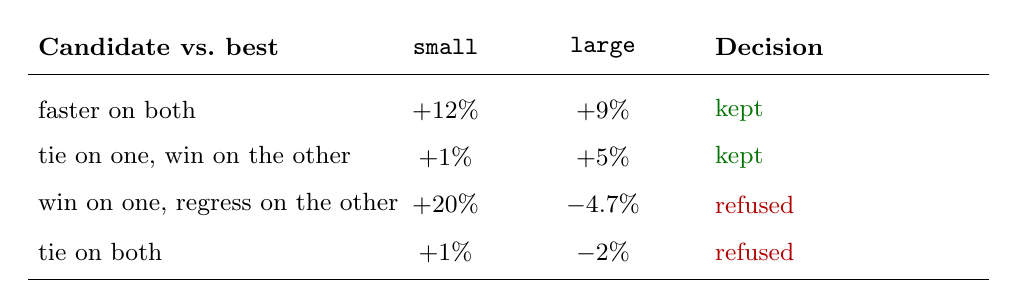
\begin{tikzpicture}[x=1cm,y=1cm]
  \def\row#1#2#3#4#5{%
    \node[anchor=west, font=\small] at (0,#1) {#2};
    \node[font=\small] at (5.3,#1) {#3};
    \node[font=\small] at (7.3,#1) {#4};
    \node[anchor=west, font=\small] at (8.6,#1) {#5};}
  \node[anchor=west, font=\small\bfseries] at (0,0.8) {Candidate vs.\ best};
  \node[font=\small\bfseries] at (5.3,0.8) {\cmd{small}};
  \node[font=\small\bfseries] at (7.3,0.8) {\cmd{large}};
  \node[anchor=west, font=\small\bfseries] at (8.6,0.8) {Decision};
  \draw (0,0.45) -- (12.2,0.45);
  \row{0}{faster on both}{$+12\%$}{$+9\%$}{\textcolor{green!45!black}{kept}}
  \row{-0.6}{tie on one, win on the other}{$+1\%$}{$+5\%$}{\textcolor{green!45!black}{kept}}
  \row{-1.2}{win on one, regress on the other}{$+20\%$}{$-4.7\%$}{\textcolor{red!70!black}{refused}}
  \row{-1.8}{tie on both}{$+1\%$}{$-2\%$}{\textcolor{red!70!black}{refused}}
  \draw (0,-2.15) -- (12.2,-2.15);
\end{tikzpicture}
\caption{The commit rule with a noise floor $\varphi = 3\%$ (the \cmd{fuzzysearch} setting).
Positive values are improvements after direction normalization. A change inside $\pm\varphi$ is a
tie. A win on one config cannot pay for a loss on another, and a tie on every config is not
progress. The third row matches the one real refusal in \cref{sec:eval}.}
\label{fig:commit-rule}
\end{figure}

\paragraph{The opt-in mean rule.} With \cmd{reduce = "mean"}, weights $w_c \geq 0$ (default 1) and
$W = \sum_{c \in \cfgs_t} w_c$, let $M(s) = W^{-1}\sum_{c\in\cfgs_t} w_c s_c$. The candidate is
accepted if the preconditions \eqref{eq:dir}--\eqref{eq:cfg} hold, $W > 0$, and the relative change
of $M$ exceeds $\varphi$. Per-config verdicts are still stored, so a regression that the mean accepts
stays visible. Dominance is the default because ``a mean lets a large win on one config pay for a
regression on another''.

\paragraph{Noise.} $\varphi$ is a \emph{relative} band applied in both directions. Noise inside the
band can neither commit nor block. A regression outside the band still blocks a gain inside it.
avocode has no repeated sampling or confidence interval in the rule; $\varphi$ is the only noise
mechanism, and it should come from measured spread. For \cmd{fuzzysearch}, the scripted reference
steps showed 0--2.5\% interquartile spread, which set $\varphi = 0.03$.

\subsection{Properties of the rule}

\begin{proposition}[Monotone lineage]
\label{prop:monotone}
With $\varphi = 0$ and \cmd{reduce = "dominate"}, for every config $c$ and every pair of versions
$i < j$ that both measure $c$, $s_c(x_j) \geq s_c(x_i)$ (as recorded at commit time).
\end{proposition}
\begin{proof}
By \eqref{eq:cfg}, a config measured by $x_i$ is measured by every later version. By
\eqref{eq:noreg} with $\varphi = 0$, each step does not decrease $s_c$. Induction on $j - i$.
\end{proof}

Three consequences follow, and the implementation relies on each.
\begin{itemize}[leftmargin=*,itemsep=1pt]
  \item \textbf{Best $=$ newest.} \avo{best} returns the version with the highest number, with no
    ranking pass. This is correct only because of \cref{prop:monotone}.
  \item \textbf{Configs only grow.} $\cfgs_t \subseteq \cfgs_{t+1}$. A new config enters with no
    baseline and is binding for every later version. A scorer edit that drops a slow config is
    refused as \cmd{missing-configs}.
  \item \textbf{The direction is frozen.} A flip is refused with the advice to ``start a fresh
    lineage rather than reinterpreting the old scores''.
\end{itemize}
With $\varphi > 0$ the guarantee weakens to $s'_c \geq s_c - \varphi|s_c|$ per step, so a chain of
small in-band losses can drift down on one config over many versions. With the mean rule, only $M$
is monotone. avocode does not re-check these properties; they hold by construction.

\paragraph{Departure from the paper.} The paper keeps a version that ``matches or improves''.
avocode requires a strict gain on at least one config. It also never re-measures the incumbent: the
best version's vector comes from its stored trailer, while the candidate is measured on today's
machine. \Cref{sec:discussion} discusses both choices.

\subsection{Guarding \texorpdfstring{$\f$}{f} against gaming}
\label{sec:gaming}

An optimizer that can edit its own objective will. \Cref{tab:gaming} lists the threats that
avocode considers and how each one is handled. Some are enforced by code. Others rest on
convention: rules in \file{AGENTS.md} and the skills. The gap matters. \avo{commit} stages with
\cmd{git add -A}, so an edit to \file{.avo/score} is committed with the candidate. A scorer edit that
drops a config or flips the direction is caught. A scorer edit that simply inflates its numbers is
not caught by the harness. The benchmarks close part of this gap with a hash gate over protected
files inside the scorer and an external audit after the run (\cref{sec:eval-bench}).

\begin{table}[t]
\centering\small
\caption{Threats to the integrity of $\f$ and how avocode handles them.}
\label{tab:gaming}
\begin{tabularx}{\linewidth}{@{}X X l@{}}
\toprule
Threat & Mechanism & Kind \\
\midrule
Commit a number that was not measured & \avo{commit} always re-scores & enforced \\
Fast but wrong candidate & $\pass$ gate before any ranking & enforced \\
A win on one config pays for a loss & dominance is the default & enforced \\
Improve by dropping a slow config & \eqref{eq:cfg}: \cmd{missing-configs} & enforced \\
Flip the metric direction & \eqref{eq:dir}: \cmd{direction-changed} & enforced \\
Noise commits a non-change & floor $\varphi$ & enforced, opt-in \\
A typo in the config disables the gate & malformed config $\Rightarrow$ all defaults & enforced \\
Hand-written version commit & only trailer-bearing commits count & convention \\
Edit \file{.avo/score} to pass & rules in \file{AGENTS.md} and skills; bench hash gate & convention / bench \\
Edit \file{lineage/} & rules; the comparator never reads \file{lineage/} & convention + design \\
\bottomrule
\end{tabularx}
\end{table}

\subsection{Persisting a version}

A version exists if and only if a commit reachable from \cmd{HEAD} carries a valid
\cmd{Avo-Version} trailer and a valid \cmd{Avo-Score} trailer. Nothing else defines a version. The
commit message has three paragraphs:
\begin{lstlisting}
avo v3: 0.408 ms

partition (pigeonhole) hash index: cut each word into k+1 segments ...

Avo-Version: 3
Avo-Score: {"primary":0.408,"unit":"ms","higher_is_better":false,
            "scores":{"small":0.309,"large":0.507}}
\end{lstlisting}
Each version has three records with different jobs (\cref{fig:records}).
\begin{enumerate}[leftmargin=*,itemsep=1pt]
  \item \textbf{The commit and its trailers}: exactly what the comparator reads back, and nothing
    more. A damaged note or a deleted Markdown file cannot change a decision.
  \item \textbf{A git note} under \cmd{refs/notes/avo}: the full attempt, logs and per-config deltas.
  \item \textbf{\file{lineage/vNNN.md}}: a readable page with the score table, parent, rationale and
    diffstat. This page is also part of $\K$ (\cref{sec:knowledge}).
\end{enumerate}
The lineage is read with one \cmd{git log} using ASCII unit and record separators. Rules for
robustness: the last trailer wins (a rebase can prepend an old body), malformed trailers are skipped
with a warning, and for duplicate numbers the newest commit wins. Because the lineage is read from
the ancestry of \cmd{HEAD}, each branch carries its own lineage.

\begin{figure}[t]
\centering
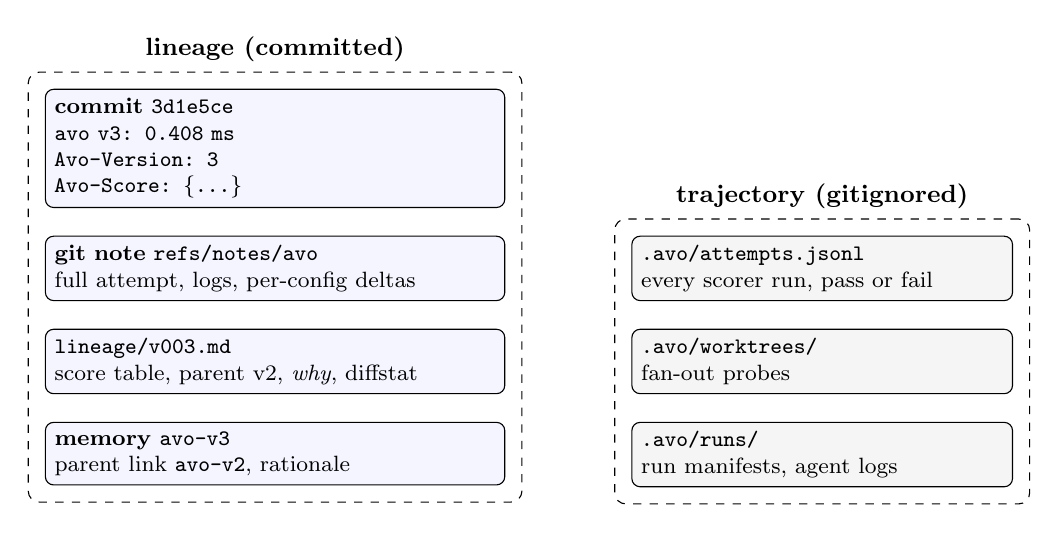
\begin{tikzpicture}[node distance=0.35cm]
  \node[store, text width=5.6cm] (c) {\textbf{commit} \texttt{3d1e5ce}\\
    \texttt{avo v3: 0.408 ms}\\ \texttt{Avo-Version: 3}\\ \texttt{Avo-Score: \{...\}}};
  \node[store, text width=5.6cm, below=of c] (n) {\textbf{git note} \texttt{refs/notes/avo}\\
    full attempt, logs, per-config deltas};
  \node[store, text width=5.6cm, below=of n] (l) {\textbf{\file{lineage/v003.md}}\\
    score table, parent v2, \emph{why}, diffstat};
  \node[store, text width=5.6cm, below=of l] (m) {\textbf{memory} \texttt{avo-v3}\\
    parent link \texttt{avo-v2}, rationale};
  \node[draw, dashed, rounded corners, fit=(c)(n)(l)(m), inner sep=6pt,
        label={[font=\small\bfseries]above:lineage (committed)}] (L) {};
  \node[store, fill=gray!8, text width=4.6cm, right=1.6cm of n] (a) {\file{.avo/attempts.jsonl}\\
    every scorer run, pass or fail};
  \node[store, fill=gray!8, text width=4.6cm, below=of a] (w) {\file{.avo/worktrees/}\\ fan-out probes};
  \node[store, fill=gray!8, text width=4.6cm, below=of w] (r) {\file{.avo/runs/}\\ run manifests, agent logs};
  \node[draw, dashed, rounded corners, fit=(a)(w)(r), inner sep=6pt,
        label={[font=\small\bfseries]above:trajectory (gitignored)}] (T) {};
\end{tikzpicture}
\caption{Lineage versus trajectory, for version v3 of the \cmd{fuzzysearch} run. The lineage
records accepted versions. The trajectory records how they were reached. Memory is committed in
the JSONL fallback and lives in the beads database otherwise.}
\label{fig:records}
\end{figure}

\paragraph{Lineage versus trajectory.} avocode keeps \emph{what survived} apart from \emph{how it was
reached}. Trajectory paths are gitignored and also unstaged after \cmd{git add -A}, in case a repo
already tracked them. avocode's own files are also excluded from the dirty check. Without this, the
memory record written after v1 would make the next turn see a change the agent never made, score it,
refuse it, record the refusal, and dirty the tree again. The project calls this class of bug
\emph{self-perturbation}; it appeared in three separate development slices.

\subsection{What happens on refusal}
\label{sec:refusal}

A refused candidate leaves no trace in git. It is recorded in three other places.
\begin{enumerate}[leftmargin=*,itemsep=1pt]
  \item \textbf{Trajectory}: the attempt is already in \file{.avo/attempts.jsonl}.
  \item \textbf{Memory}: a dead-end record keyed by content,
    $\mathit{key} = \mathrm{sha256}(\mathit{reason} \,\|\, \mathit{vector})_{[0:8]}$, so a repeat of
    the same dead end updates one record instead of adding a new one.
  \item \textbf{Output}: the reason names the configs and deltas, for example \emph{``\,`small'
    regressed (worst: small $-4.74\%$) (floor $\pm 3.00\%$)''}.
\end{enumerate}
Harness errors are \emph{not} recorded as dead ends, because ``a harness error taught us nothing
about the candidate''. The refused candidate stays in the working tree, so the agent can keep
working on it. The skill tells the agent to add an insight with \avo{mem add} when it knows
\emph{why} a change failed, because ``an unrecorded refusal is one the next session earns again''.

\subsection{Memory}

The paper's agent remembers through its conversation history. avocode moves memory out of the agent
and into the repository, which is what makes the operator restartable and agent-agnostic. A memory
record has the shape \cmd{\{ts, kind, key, text, version, parent\}}, with four kinds:
\cmd{insight}, \cmd{version}, \cmd{failure} and \cmd{intervention}. If the beads issue tracker
\citep{yegge2025beads} is present, records become beads, and version records are linked parent to
child, which mirrors the lineage as a dependency graph. Otherwise they go to
\file{lineage/memory.jsonl}, append-only with last-write-wins per key. The agent reads the same JSON
in both cases. \avo{mem prime} prints insights, ``dead ends (do not re-try these)'' and committed
versions. Interventions are left out on purpose, so old directives do not echo into new sessions.

\subsection{Knowledge \texorpdfstring{$\K$}{K}}
\label{sec:knowledge}

$\K$ has two Markdown collections: \file{knowledge/} (``what we were told'': docs and papers) and
\file{lineage/} (``what we learned''). Both are indexed by qmd \citep{lutke2025qmd}, which combines BM25,
vector search, LLM query expansion and a local reranker. Because \avo{commit} already writes
\file{lineage/vNNN.md}, the question ``what did I already try about register pressure?'' is the same
query as ``what do the docs say about it?''. This turns the paper's observation that the agent
``frequently examines multiple prior implementations in $\Pt$'' into a single search over both.

Without a project-local qmd index, a local scan returns the same JSON shape. Its score is the
fraction of distinct query terms that match, and it says it is not BM25. Documents can be added from
the web with \avo{know search --ingest} or \avo{know add}. Each added file records its
\cmd{source}, \cmd{title}, \cmd{fetched-at} time and \cmd{via} backend in front matter, so a
claim in $\K$ can be traced and checked later. Re-adding a page with the same body is a no-op; a
different body is refused without \cmd{--force}.

\section{Orchestration}
\label{sec:orchestration}

\subsection{The variation step as a skill}

The \cmd{avo-vary} skill tells the agent: ``You are the variation operator \ldots\ You do
\emph{not} decide what gets kept --- \avo{commit} does.'' It prescribes one step in a fixed order:
\begin{lstlisting}
avo mem prime                 # 1. what past turns learned, incl. dead ends
avo best; avo lineage         # 2. the version to beat, and the whole population
avo know query "<the idea>"   # 3. K: docs and prior lineage entries
# 4. make ONE coherent change
avo score --json              # 5. measure it
avo commit --why "<what changed and why it should help>"
\end{lstlisting}
Steps 1--3 are the agent's reading of $\Pt$ and $\K$ in \cref{eq:intro-agent}. The rule ``one idea
per candidate'' makes a refusal attributable to one change. Inside this step the agent is free: it
can profile, read code, search the web, or call \avo{fan} (\cref{sec:fan}). This is the paper's
edit--evaluate--diagnose cycle, written as instructions rather than code.

\subsection{\texorpdfstring{\avo{run}}{avo run}: the continuous loop}
\label{sec:run}

\avo{run} automates the cycle of \cref{fig:loop}. Its central choice differs from the paper:
\emph{each turn is a fresh agent process}. The paper's agent keeps one conversation for seven days.
In avocode, ``every iteration is a fresh process, so the turn prompt is the only continuity''. All
other state lives in the repository: the lineage in git, the trajectory in the attempt log, and
memory in beads or JSONL. \Cref{alg:run} gives the loop.

\begin{algorithm}[t]
\caption{\avo{run}: the outer loop}
\label{alg:run}
\begin{algorithmic}[1]
\Require repo with seed commit $x_0$; prompt $\pi$; agent $\alpha$; budget $T$; turn timeout $\tau$;
  thresholds $N$ (stall), $R$ (thrash)
\State \Call{CheckGuards}{$\pi$} \Comment{depth $<$ cap, $\mathrm{sha}(\pi) \notin$ chain}
\State $d \gets \bot$;\ $\mathit{prev} \gets \bot$;\ $\mathit{idle} \gets 0$
\For{$t = 1, \ldots, T$}
  \If{\file{.avo/STOP} exists} \Return \textsc{stop-file} \EndIf
  \State $h_0 \gets \texttt{HEAD}$
  \State $p \gets \Call{TurnPrompt}{\pi, t, \mathit{prev}, d}$ \Comment{$\pi$ verbatim at $t=1$}
  \State $(\mathit{ok}, \mathit{summary}) \gets \Call{DriveAgent}{\alpha, p, \tau}$
    \Comment{fresh process: $\Vary(\Pt)$}
  \If{spawn failed} \Return \textsc{agent-unavailable} \EndIf
  \State $\mathit{dec} \gets \Call{Commit}{\mathit{summary}}$ \Comment{\cref{alg:commit}; summary becomes \emph{why}}
  \State $h_1 \gets \texttt{HEAD}$;\ credit versions in $h_0..h_1$ \Comment{agent may commit itself}
  \State $\mathit{idle} \gets (\mathit{dec} = \textsc{noop} \wedge h_1 = h_0)\ ?\ \mathit{idle}+1 : 0$
  \State $(\mathit{sig}, d) \gets \Call{Supervise}{N, R}$ \Comment{\cref{alg:supervise}}
  \If{$\mathit{sig} \neq \emptyset$} record an \cmd{intervention} memory \EndIf
  \State write manifest \Comment{after every iteration}
  \State $\mathit{prev} \gets (\mathit{dec}, \mathit{sig})$
  \If{$\mathit{idle} \geq 3$} \Return \textsc{no-progress} \EndIf
\EndFor
\State \Return \textsc{max-iters}
\end{algorithmic}
\end{algorithm}

\begin{algorithm}[t]
\caption{\textsc{Commit}($\mathit{why}$): the only writer of $\Pt$}
\label{alg:commit}
\begin{algorithmic}[1]
\If{tree is clean, ignoring harness paths} \Return \textsc{noop} \EndIf
\State $a \gets \f(\text{working tree})$;\ append $a$ to the attempt log
\State $b \gets$ newest version in $\Pt$ \Comment{best, by \cref{prop:monotone}}
\If{$a$ has harness errors} \Return \textsc{error} \EndIf
\If{$\neg\pass(a)$ \textbf{or} ($b \neq \bot$ \textbf{and not} \Call{Accept}{$a, b$})} \Comment{\cref{def:commit}}
  \State record dead end, key $= \mathrm{sha256}(\mathit{reason}\,\|\,\mathit{vector})$
  \State \Return \textsc{refused}
\EndIf
\State commit with trailers; add git note; write \file{lineage/vNNN.md}; record version memory
\State \Return \textsc{committed}
\end{algorithmic}
\end{algorithm}

\paragraph{The turn prompt.} The first turn gets the operator's prompt verbatim. Later turns get the
prompt plus a footer: the turn number, a one-line outcome of the previous turn (for example
\emph{``committed v3 at 0.408 ms''} or \emph{``refused at 0.42 ms --- \ldots''}), the number of
attempts since the best version, a reminder that the agent is a fresh process that should read
\avo{lineage}, \avo{best} and \avo{mem prime}, and the supervisor's directive if one fired. The
directive is \emph{appended} to the task, never substituted for it.

\paragraph{Committing.} The agent's final message, capped at 2{,}000 characters, becomes the
\emph{why} of the commit. The skill also allows the agent to call \avo{commit} itself during the
turn. The harness therefore reads the trailers in $h_0..h_1$ and credits those versions too. Before
this fix, a run that grew four versions reported that it had committed none.

\paragraph{Termination.} The loop stops on the iteration budget, on a \file{.avo/STOP} file, after
three consecutive idle turns, or when the agent binary cannot start. The stop file needs no process
to find, and the agent can create it when the task is done. The idle rule exists because ``an
unchanged tree records no attempt, so the stall detector cannot see it''. A timed-out turn does not
stop the loop; its process group is killed and the next turn starts. The supervisor never stops the
loop. It only steers.

\paragraph{Crash safety.} The run manifest is the same object as the \cmd{--json} report, and it is
rewritten after every iteration: ``a days-long loop gets killed eventually, and per-iteration versus
at-exit is a recoverable record versus nothing''. There is no \cmd{--resume}. Recovery is structural:
each version is committed before the next turn, so a new \avo{run} with the same prompt continues
from \cmd{HEAD}. The second benchmark run in \cref{sec:eval} did exactly this.

\paragraph{Budgets.} \avo{run} has an iteration budget and a per-turn timeout (default 900\,s). It
has no wall-clock budget and no cost budget. Cost is recorded but not enforced.

\subsection{\texorpdfstring{\avo{supervise}}{avo supervise}: stagnation detection}
\label{sec:supervise}

The paper's supervisor is an agent. avocode's supervisor is a pure function of what the harness
already records, plus a text template. It makes no LLM call. The design reason is in the source:
\begin{quote}\small
``The output is a directive that \textbf{cites}. `Try something else' is worthless --- the agent
already believes it is.''
\end{quote}
It detects two signals. Let $A = (a_1, \ldots, a_m)$ be the last 1{,}000 attempts, newest last, and
$b$ the best version.

\begin{definition}[Stall]
Let $s = |\{a \in A : \mathrm{head}(a) = \mathrm{sha}(b) \vee \mathrm{ts}(a) \geq \mathrm{date}(b) +
1\,\mathrm{s}\}|$, or $s = m$ if no version exists. Stall fires when $s \geq N$ and $s > 0$, with
$N = 5$ by default.
\end{definition}
\noindent Attempts are matched to $b$ by git \cmd{HEAD} first, not by clock: the attempt that
\emph{became} $b$ was scored before the commit and carries the parent's SHA, and git truncates
commit dates to the second. An attempt that passed $\f$ but did not beat $b$ still counts.

\begin{definition}[Thrash]
Let $\mathrm{sig}(a)$ be the failure signature of $a$, or $\bot$ for a passing attempt. Let $r$ be the
length of the longest suffix of $A$ whose signatures all equal $\mathrm{sig}(a_m) \neq \bot$. Thrash
fires when $r \geq R$, with $R = 3$ by default.
\end{definition}
\noindent The signature is the first harness error, else the scorer's first log line, normalized so
that noise does not split one failure into many: lowercase; temporary paths, hex SHAs and numbers
replaced by placeholders; whitespace folded; truncated to 200 characters. A pass breaks the streak.
Thrash ``usually means the diagnosis is wrong rather than the edit''.

There is no test for a score plateau, for repeated ideas, or for similarity between a candidate and
prior versions. The harness ranks measurements, not ideas. Novelty is left to the agent, which the
directive gives the evidence to judge.

\paragraph{The directive.} Only when a signal fires does the supervisor read memory and $\K$, so the
common case stays cheap. The directive cites:
\begin{itemize}[leftmargin=*,itemsep=1pt]
  \item up to three recent versions, with score, rationale and lineage file (``a variation that only
    re-derives one of these is not progress'');
  \item up to five memories, dead ends before insights;
  \item up to three documents in $\K$ that no version or memory has mentioned.
\end{itemize}
A document $d$ with significant title terms $T(d)$ counts as \emph{unexplored} against the corpus
$C$ of all version rationales and memories when
\begin{equation}
  2\,\big|\{u \in T(d) : u \in C\}\big| < |T(d)|.
\end{equation}
The bar is low on purpose: a document wrongly marked explored costs one citation, while one wrongly
marked unexplored ``sends the agent back down a road it already travelled''. Interventions are never
cited. Citing them would nest old directives inside new ones, and would put every recommended
document name into the corpus, so ``it would erase its own best advice''. \Cref{fig:directive} shows
a real directive from a test fixture.

\begin{figure}[t]
\begin{lstlisting}
STEERING (avo supervise)

- stall: 5 attempt(s) since v1 (16 bytes) with no committed improvement; the threshold is 5

Already committed (a variation that only re-derives one of these is not progress):
  - v1 - 16 bytes - shrink the kernel by removing five redundant bytes (lineage/v001.md)

In K and never mentioned by any version - unexplored:
  - knowledge/loop-tiling.md - Loop tiling and cache blocking
  - knowledge/register-pressure.md - Register pressure on Blackwell

Do this next:
  1. Name the direction you are about to take, and say how it differs from every line
     above. If you cannot, you do not have a new idea yet.
  2. Change one thing, then `avo score` before you change a second.
  3. `avo commit --why "<the direction>"` when it measures better. A refusal is a
     measurement: record it with `avo mem add`, do not retry it.
  4. If every direction you can name is already above, do not guess: `avo fan --n 4`
     explores four at once and lets f choose.
\end{lstlisting}
\caption{A stall directive (abridged), generated in a fixture repository with one version, five
attempts that did not beat it, and two documents in $\K$. When thrash fires, step 1 instead says
that ``the same error $N$ times means the \emph{diagnosis} is wrong, not the edit''.}
\label{fig:directive}
\end{figure}

\begin{algorithm}[t]
\caption{\textsc{Supervise}($N, R$)}
\label{alg:supervise}
\begin{algorithmic}[1]
\State $A \gets$ last 1000 attempts;\ $b \gets$ newest version
\State $s \gets |\{a \in A : \mathrm{head}(a) = \mathrm{sha}(b) \vee \mathrm{ts}(a) \geq \mathrm{date}(b) + 1\mathrm{s}\}|$
\State $r \gets$ longest suffix of $A$ with one non-null signature
\State $\mathit{sig} \gets \{\textsc{stall} \mid s \geq N \wedge s > 0\} \cup \{\textsc{thrash} \mid r \geq R\}$
\If{$\mathit{sig} = \emptyset$} \Return $(\emptyset, \bot)$ \EndIf
\State $V \gets$ newest 3 versions;\ $F \gets$ up to 5 memories (dead ends first, no interventions)
\State $U \gets$ up to 3 documents in $\K$ that are unexplored
\State \Return $(\mathit{sig}, \Call{Render}{\mathit{sig}, V, F, U})$ \Comment{$\leq 4000$ characters}
\end{algorithmic}
\end{algorithm}

\paragraph{Two delivery paths.} In \avo{run}, the directive enters the \emph{next} turn's prompt and
is recorded as an \cmd{intervention} memory. In the pi agent, an extension runs the same detector
after every \cmd{avo\_score} or \cmd{avo\_commit} tool result and injects the directive into the
\emph{current} session as a steering message. It sends one directive per episode: an episode key
built from the best version's SHA and the start of the streak makes ``5 since best'' and ``6 since
best'' the same episode. Its state is rebuilt from the session branch, so a branched session that
never saw a directive gets one. Both paths count the attempt log, not the session: ``two drifting
counters would steer one stall twice''.

\subsection{\texorpdfstring{\avo{fan}}{avo fan}: parallel probes}
\label{sec:fan}

\avo{fan} explores $N$ directions at once. Each probe gets its own detached git worktree at
\cmd{HEAD} and its own headless agent process. The probes run on a small model (set by
\cmd{AVO\_PROBE\_MODEL}), because ``exploration is a small-model job, exploitation is a big-model
job''. \avo{run} uses the agent's default model. All probes get the \emph{same} prompt; diversity
comes from sampling. The skill therefore asks for a prompt that names the problem, not the edit:
``delete the bounds check'' gives $N$ identical diffs.

Each probe is scored in its worktree without writing to the root attempt log, so probes never
trigger the supervisor. A probe is scored even if its agent failed, since ``a half-finished edit
passing $\f$ is a real result''. Worktrees with no changes are removed. The manifest is written after
every probe, so \cmd{--resume} reruns only unfinished probes after a crash.

\paragraph{Selection.} Let $\nu(x) = \mathrm{primary}(x)$ if higher is better and $-\mathrm{primary}(x)$
otherwise. The harness computes
\begin{equation}
  \hat{\imath} = \operatorname*{arg\,max}_{i\,:\,\pass(x_i)} \nu(x_i),
  \qquad \hat{\imath} = \bot \text{ if no probe passes},
\end{equation}
with ties going to the smallest index. This is ``a hint, never a decision''. Promotion is manual:
\avo{fan --promote} $j$ saves and applies probe $j$'s diff to the root tree and stops. The candidate
must then go through \avo{score} and \avo{commit}, which re-measures it in the real tree:
\begin{equation}
  x_{t+1} =
  \begin{cases}
    \mathrm{promote}(x_j) & \text{if the commit rule accepts it against } x_t,\\
    x_t & \text{otherwise.}
  \end{cases}
\end{equation}
The skill allows at most one promotion per step, because ``two probes' diffs stacked together is a
candidate neither of them measured''.

\paragraph{Recursion guards.} A probe is an agent with the same skills, so it can call \avo{fan}
itself, and a turn of \avo{run} can call \avo{run}. Four guards bound this, carried in environment
variables, ``the only channel surviving \cmd{spawn} into an arbitrary agent binary'':
\begin{enumerate}[leftmargin=*,itemsep=1pt]
  \item \textbf{Depth}: refuse when the level reaches the cap (default 3); a child gets level $+1$.
  \item \textbf{Cycle}: refuse when the prompt's hash is already in the chain of ancestors.
  \item \textbf{Concurrency}: at most $\min(8, \mathit{cpus} - 2)$ probes at once.
  \item \textbf{Timeout}: 900\,s per probe, after which the whole process group is killed.
\end{enumerate}
A guard refusal is exit 1, not 2: ``a guard is a refusal, not a harness failure''. avocode uses OS
processes and worktrees, not in-process sub-agents, because the design notes judge that sub-agent
extensions ``do not work well enough''.

\subsection{Agent adapters}
\label{sec:adapters}

One function, \cmd{driveAgent}, runs one headless turn for both \avo{run} and \avo{fan}.
\Cref{tab:adapters} lists the templates. Every flag was read off the real binaries, because ``a
wrong flag fails silently''. The prompt follows \cmd{--}, so a prompt that starts with a dash is not
read as a flag. Token counts are normalized to four disjoint fields: uncached input, output, cache
read and cache write. Codex reports cached input as a subset of input, so it is subtracted.

\begin{table}[t]
\centering\small
\caption{Headless agent templates. A custom template can be set in \file{.avo/config.json}.}
\label{tab:adapters}
\begin{tabularx}{\linewidth}{@{}l X X@{}}
\toprule
Agent & Command & Skill discovery \\
\midrule
pi \citep{zechner2025pi} & \cmd{pi --mode json --print --approve -- <prompt>} & native \file{.agents/skills/}; six native tools; in-session supervisor \\
Claude Code \citep{anthropic2025claudecode} & \cmd{claude --print --output-format stream-json --verbose --permission-mode bypassPermissions -- <prompt>} & \file{.claude/skills} $\to$ \file{.agents/skills} symlink \\
Codex \citep{openai2025codex} & \cmd{codex exec --json --skip-git-repo-check --sandbox workspace-write -- <prompt>} & skills index in \file{AGENTS.md} \\
\bottomrule
\end{tabularx}
\end{table}

\avo{install} wires the skills into a target repository by \emph{linking}, never copying: ``a copy is
a fork that stops receiving fixes''. It validates each skill against the Agent Skills
specification first, because pi is lenient, Claude Code is strict, and a skill must load everywhere.
It also writes a managed block into \file{AGENTS.md} with the rules and a skills index, and leaves
text outside the markers alone.

For pi, an extension adds six native tools (\cmd{avo\_score}, \cmd{avo\_commit},
\cmd{avo\_lineage}, \cmd{avo\_know\_query}, \cmd{avo\_know\_add}, \cmd{avo\_fan}). They are thin
wrappers over the same functions as the CLI. A refusal is a normal result, not an error. No tool
takes a working directory, because ``an agent that can retarget the repo can write a version into a
repo nobody is watching''.

\section{Evaluation}
\label{sec:eval}

The evaluation asks three questions. Does the loop make real progress on a target it has not seen?
Does the commit rule keep the lineage honest? And what does a turn cost? All numbers below come from
transcripts committed in the repository (\file{evidence/}) and from the design log
(\file{PLAN.md}).

\subsection{Benchmarks}
\label{sec:eval-bench}

The repository ships two targets in \file{bench/}, chosen to be unlike each other
(\cref{tab:bench}). \cmd{fuzzysearch} is a speed problem with a known answer, so it tests the
harness. \cmd{arcagi3} is an open capability problem, so it tests the loop. A script copies a target
into a fresh git repository and refuses any path inside the avocode checkout, because \avo{commit}
would otherwise write the loop's lineage into avocode's own history.

\begin{table}[t]
\centering\small
\caption{The two benchmark targets. Both use \cmd{reduce = "dominate"}.}
\label{tab:bench}
\begin{tabularx}{\linewidth}{@{}l X X c c c@{}}
\toprule
Target & Task & \cmd{primary} & Dir. & Configs & $\varphi$ \\
\midrule
\cmd{fuzzysearch} & all (query, word) pairs with Levenshtein distance $\leq k$ & mean of per-config median ms per search & $\downarrow$ & 2 & 0.03 \\
\cmd{arcagi3} & play ARC-AGI-3 games \citep{arcprize2026arcagi3} from $64{\times}64$ frames & mean fraction of levels completed & $\uparrow$ & 10 & 0.1 \\
\bottomrule
\end{tabularx}
\end{table}

\paragraph{\cmd{fuzzysearch}.} Two configs, \cmd{small} (2{,}500 words, 80 queries) and
\cmd{large} (5{,}000 words, 120 queries), both with $k = 2$, are built from a seeded pseudo-lexicon
so they are identical on every machine. The repetition count adapts to the candidate's speed. Spread
is measured as an interquartile range, because max-minus-min showed 51\% ``spread'' at the fast end
from one garbage-collection pause. The seed program is a full dynamic-programming matrix built from
nested arrays: correct and slow. The scorer's \cmd{correct} has three gates, in order:
\begin{enumerate}[leftmargin=*,itemsep=1pt]
  \item \textbf{Hash gate}: \cmd{sha256sum -c} over the protected files (the reference, corpus,
    runner, unit tests, the scorer and the protected list itself).
  \item \textbf{Unit suite}: empty inputs, $k=0$, exact distances, Unicode, duplicates.
  \item \textbf{Full-scale check}: compare the candidate with an independent reference on the
    exact input that is timed, and check that the candidate did not mutate its arguments.
\end{enumerate}
Gate~3 matters. The end-to-end suite ships a candidate that passes every unit test but returns
nothing for corpora over 1{,}000 words. Only gate~3 catches it (``306 pair(s) missing''). An agent
that edits both the scorer and the hash file can defeat the in-repo gate, so an external
\cmd{bench/init.sh --verify} audits the protected files from outside the target after each run.

Before any agent ran, six hand-written versions (the \emph{ladder}) were replayed through
\avo{score} and \avo{commit} to prove that the target has headroom: two-row DP, length prefilter,
prefix/suffix trim, an Ukkonen band, a length-bucketed index, and a letter-set bitmask. All six
committed, and the ladder went from \SI{1719}{ms} to \SI{0.931}{ms} ($1847\times$) in the committed
transcript. A first candidate target, matrix multiplication, was rejected at this stage: five
classical optimizations gave only $1.7\times$ in total, because the V8 JIT already does that work.

\paragraph{\cmd{arcagi3}.} A policy plays ten offline ARC-AGI-3 games with a budget of 250 actions
per episode and 24 seeded rollouts per game. Games were removed if their baseline was zero, if they
were not reproducible (a real-time game scored 0.483, 0.533 and 0.483 on identical code), or if they
were saturated. The scorer adds a sandbox through Python audit hooks that refuses network access and
reads of the game files while the policy acts. An earlier version raised a plain \cmd{Exception},
and ``a policy wrapping its body in \texttt{except Exception: pass} swallowed the violation and
scored a clean 0.26''. Eight held-out games and the official API are scored outside $\f$, because
memorization is the one thing $\f$ cannot catch. A scripted two-rung ladder moves the training score
from 0.277 to 0.320 and the holdout from 0.217 to 0.227; its second rung is refused because one game
drops by 100\%. \textbf{No agent run on \cmd{arcagi3} is recorded}, so we report it as a built and
gated target, not as a result.

\subsection{Setup of the agent runs}

Both runs used \avo{run --agent claude} with Claude Code's default model on one workstation. $\K$
was seeded with four notes written offline: Ukkonen's banded DP, Myers' bit-parallel algorithm,
BK-trees with Levenshtein automata, and V8 numeric-loop performance. The notes ``deliberately do not
contain the ladder''. qmd and web search were not available, so $\K$ used the local-scan fallback. A
watchdog created \file{.avo/STOP} after a fixed time (1{,}500\,s for run~1, 1{,}200\,s for run~2), so
\textbf{both runs stopped on the clock, not on convergence}. Run~2 resumed the lineage of run~1 with
the same prompt. Before it started, the operator removed run~1's refused candidate from the working
tree and saved it as evidence. \Cref{tab:runs} lists the settings.

\begin{table}[t]
\centering\small
\caption{Settings and outcomes of the two agent runs on \cmd{fuzzysearch}.}
\label{tab:runs}
\begin{tabular}{@{}lcc@{}}
\toprule
 & Run 1 & Run 2 (resumed) \\
\midrule
Turns (budget)            & 6 (12) & 3 (6) \\
Per-turn timeout          & 480\,s & 900\,s \\
Wall-clock                & 34\,min 43\,s & 30\,min 41\,s \\
Stopped by                & watchdog & watchdog \\
Versions committed        & 4 (v1--v4) & 3 (v5--v7) \\
Refusals                  & 1 & 0 \\
Supervisor interventions  & 0 & 0 \\
Cost                      & $\geq$ \$1.91 (2 of 6 turns recoverable) & \$8.19 (\$2.73/turn) \\
$\f$ intact (external audit) & pass & pass \\
\bottomrule
\end{tabular}
\end{table}

\subsection{Results}

\Cref{tab:lineage,fig:results} give the lineage. Seven versions took the median search time from
\SI{1810.37}{ms} to \SI{0.231}{ms}, a $7837\times$ speedup, in nine turns and about 65 minutes of
agent time. Run~1 alone reached $5255\times$ in four versions. Every version satisfied
\cref{def:commit} against its parent with $\varphi = 3\%$, so no regression beyond the floor
was committed on either config.

\begin{table}[t]
\centering\small
\caption{The agent lineage on \cmd{fuzzysearch}. Times are medians in ms at commit time. Speedups
for v5--v7 versus v0 are computed by hand from the recorded primaries; the run transcript's ``vs
v0'' column is wrong for run~2 (it uses the run's start as v0).}
\label{tab:lineage}
\begin{tabularx}{\linewidth}{@{}c c X r r r r r@{}}
\toprule
Ver. & Run & Technique (from the commit rationale) & \cmd{small} & \cmd{large} & \cmd{primary} & vs.\ prev & vs.\ v0 \\
\midrule
v0 & -- & full DP matrix, nested arrays (seed) & -- & -- & 1810.37 & -- & $1\times$ \\
v1 & 1 & rolling \cmd{Int32Array} Ukkonen band, length-bucketed corpus, flat code units & 3.447 & 10.261 & 6.854 & $264.1\times$ & $264\times$ \\
v2 & 1 & character-set bitmask prefilter before the banded DP & 0.435 & 0.849 & 0.642 & $10.7\times$ & $2820\times$ \\
v3 & 1 & \textbf{partition (pigeonhole) hash index} --- not in the ladder & 0.309 & 0.507 & 0.408 & $1.57\times$ & $4437\times$ \\
v4 & 1 & PassJoin position-aware probe window on that index & 0.253 & 0.436 & 0.345 & $1.18\times$ & $5255\times$ \\
v5 & 2 & one interleaved \cmd{Int32Array} for the index & 0.248 & 0.413 & 0.331 & $1.04\times$ & $5478\times$ \\
v6 & 2 & Myers bit-parallel for survivors; layout fused into index build & 0.173 & 0.368 & 0.270 & $1.22\times$ & $6693\times$ \\
v7 & 2 & no flat corpus buffer; branchless Myers with early exit & 0.158 & 0.304 & 0.231 & $1.17\times$ & $7837\times$ \\
\bottomrule
\end{tabularx}
\end{table}

\begin{figure}[t]
\centering
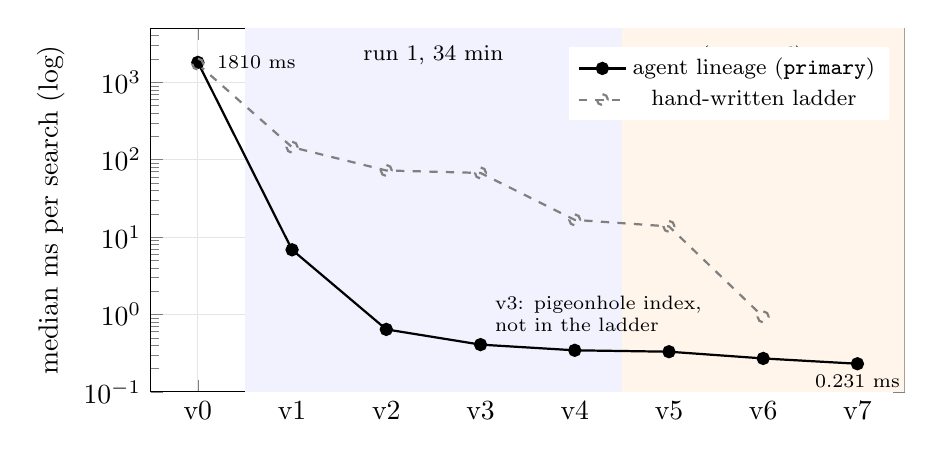
\begin{tikzpicture}
\begin{semilogyaxis}[
  width=0.92\linewidth, height=6.2cm,
  xmin=-0.5, xmax=7.5, ymin=0.1, ymax=5000,
  xtick={0,...,7}, xticklabels={v0,v1,v2,v3,v4,v5,v6,v7},
  ylabel={median ms per search (log)},
  grid=major, grid style={gray!20},
  legend style={at={(0.98,0.95)}, anchor=north east, font=\footnotesize, draw=none},
  every axis plot/.append style={thick},
]
  \fill[blue!5] (axis cs:0.5,0.1) rectangle (axis cs:4.5,5000);
  \fill[orange!8] (axis cs:4.5,0.1) rectangle (axis cs:7.5,5000);
  \node[font=\footnotesize, anchor=north] at (axis cs:2.5,4000) {run 1, 34 min};
  \node[font=\footnotesize, anchor=north] at (axis cs:6,4000) {run 2 (resumed), 31 min};
  \addplot[mark=*, black] coordinates
    {(0,1810.37) (1,6.854) (2,0.642) (3,0.408) (4,0.3445) (5,0.3305) (6,0.2705) (7,0.231)};
  \addlegendentry{agent lineage (\cmd{primary})}
  \addplot[mark=o, gray, dashed] coordinates
    {(0,1719.368) (1,145.093) (2,72.603) (3,67.434) (4,16.693) (5,13.7455) (6,0.931)};
  \addlegendentry{hand-written ladder}
  \node[font=\scriptsize, anchor=south west, align=left] at (axis cs:3.05,0.45)
    {v3: pigeonhole index,\\ not in the ladder};
  \node[font=\scriptsize, anchor=west] at (axis cs:0.1,1810) {1810 ms};
  \node[font=\scriptsize, anchor=north] at (axis cs:7,0.22) {0.231 ms};
\end{semilogyaxis}
\end{tikzpicture}
\caption{The \cmd{fuzzysearch} lineage on a log scale ($7837\times$, no committed regression). The
dashed line is the hand-written ladder from a separate transcript, shown for scale; its v0 is a
different measurement of the same seed. The ladder's last rung (\SI{0.931}{ms}) is slower than the
agent's v2.}
\label{fig:results}
\end{figure}

\paragraph{Reproduction.} An audit script re-measured every version from its own commit in a
detached worktree. All fresh measurements were slower than the recorded ones, by 0.9\% to 12.9\%,
all in one direction, because ``the box was busy''. The audit's pass band is 50\%, so all seven
versions passed. The audit also confirmed a monotone best and an intact $\f$.

\subsection{Case studies}

\paragraph{A step outside the ladder.} v1 fused five of the six ladder steps into one commit, and v2
matched the ladder's last step. v3 went further. The agent cut each corpus word into $k+1$ disjoint
segments and hashed them. By the pigeonhole principle, any match within $k$ edits keeps at least one
segment intact, so the scan becomes a few hash probes. A source comment records that this cut the
candidates from about 283k to about 23k on the scored workload. The commit rationale cites the
bucketing note in $\K$: ``the same idea applies to any filter whose key is discrete''. v4 (PassJoin
windows), v6 (Myers bit-parallel) and v7 also go beyond the ladder. The design log concludes that
``the ladder is a floor on this target, not a ceiling''. We note that the seeded notes named the
relevant algorithm families, so $\K$ shaped this result.

\paragraph{The one refusal.} In run~1, turn~6 (which hit the 480\,s timeout) left a candidate that
interleaved the index entries. It was slower than v4 on \cmd{small} by 4.74\%, outside the 3\%
floor, and the rule refused it: \emph{``\,`small' regressed (worst: small $-4.74\%$) (floor
$\pm3.00\%$)''}. In run~2, a fresh agent reached the same idea and made it win as v5: a tie on
\cmd{small} ($+2.0\%$, inside the floor) and a gain on \cmd{large} ($+5.3\%$). The dead-end record
did not block a better implementation of the same idea. It only blocked the version that
regressed.

\paragraph{A wrong note, corrected by measurement.} Each turn of run~2 started by measuring. The
turn that produced v6 timed each phase and found that the banded DP took 30--43\% of the call. Notes
from v4 and v5 had called it ``almost certainly too small to matter now''. The agent recorded that
the earlier note was wrong.

\paragraph{The rule shapes the step.} Two of the three turns in run~2 bundled changes on purpose. A
change worth $+2.66\%$ is inside the 3\% floor, so it cannot commit alone, and the agent shipped it
with a partner. The design log calls this ``the commit rule shaping the variation step''. It also
conflicts with the skill's ``one idea per candidate'' rule, which \cref{sec:discussion} discusses.

\paragraph{A dead end found twice.} The turns for v6 and v7 both tried to drop a counting sort and
both measured a regression. The second turn retried on purpose, reasoning that a later change should
have removed the first cause. It had not.

\subsection{Cost and tokens}
\label{sec:eval-cost}

Run~2 used 158 uncached input tokens, 119{,}912 output tokens, 5{,}555{,}257 cache-read tokens and
241{,}350 cache-write tokens, for \$8.19 or \$2.73 per turn. At that rate, the default budget of
12 turns costs about \$33, and \avo{run} has no cost cap. Run~1's cost is only a floor. Its
manifest recorded 44 of 985{,}039 input tokens (0.0045\%) because of two bugs: the parser read only
uncached input, and the output cap kept the head of the agent's stream while Claude Code writes usage
and cost in the last event. Four of six logs lost that event. Both bugs are fixed, and a replay tool
re-parses saved logs with the fixed parser. Bugs like this one, and an agent's own commits not being
credited to its turn, appeared only in real runs; stub agents in the test suite did not expose them.

\subsection{Engineering validation}

The repository has 441 unit tests (\cmd{node:test}, about 4.6\,s) and 14 end-to-end suites that run
the real \cmd{bin/avo} against temporary git repositories with a stub agent. Each suite writes a
transcript to \file{evidence/}; the current transcripts hold 496 passing checks. Continuous
integration runs lint, type checks, the unit tests and the end-to-end suites on every pull request,
with no agent installed on purpose. Examples of what the suites pin down: the stall fires at exactly
$N$ attempts and not before; a directive is appended to the turn prompt, not substituted; six
worsening scores in a pi session produce \emph{one} directive; a second \avo{install} produces no
diff; and a candidate that is fast but wrong at full scale fails $\f$.

The supervisor fired in these tests and \emph{never} in a real run. Across nine real turns,
attempts-since-best peaked at 2. ``A target with 5000x of headroom is improved faster than a stall
detector can notice one.''

\section{Discussion}
\label{sec:discussion}

\subsection{Fidelity to AVO}

\Cref{tab:fidelity} compares avocode with the paper, object by object. Where the paper is specific,
avocode follows it: a single lineage, versions as git commits with scores, a vector $\f$ with a
correctness gate, a knowledge base, and a supervisor for stall and unproductive cycles. Where the
paper is silent, avocode has to choose, and it chooses the stricter option each time.

\begin{table}[t]
\centering\small
\caption{avocode compared with the AVO paper.}
\label{tab:fidelity}
\begin{tabularx}{\linewidth}{@{}l X X@{}}
\toprule
Aspect & AVO paper & avocode \\
\midrule
Domain & CUDA attention kernels on B200 & any repository with \file{.avo/score} \\
$\f$ & vector of TFLOPS per config; 0 if incorrect & JSON line with optional vector; \cmd{null} if $\neg\pass$, refused before ranking \\
Acceptance & ``matches or improves'' the best; vector rule and tolerance not given & \cref{def:commit}: dominance, strict gain on one config, relative floor $\varphi$; ties refused \\
Anti-gaming & not discussed & re-score at commit; no measuring less; frozen direction; bench hash gates \\
$\Pt$ storage & git commit with its score & commit $+$ trailers $+$ git note $+$ \file{lineage/vNNN.md} \\
Failed attempts & inside the agent's context, then lost & attempt log and content-keyed dead ends, read by later sessions \\
$\K$ & CUDA/PTX docs, FA4 source & \file{knowledge/} with provenance $+$ the lineage itself, hybrid search \\
Agent & one internal agent, unnamed LLMs & pi, Claude Code or Codex via portable skills \\
Continuity & one conversation for 7 days & fresh process per turn; state in the repository \\
Supervisor & a supervisor agent; mechanism not given & deterministic stall/thrash detector; citing directive; no LLM call \\
Population & single lineage; branching is future work & single lineage $+$ \avo{fan} probes, one promoted \\
Scale of evidence & 7 days, 40 versions, $>$500 directions & 65 minutes, 7 versions, 9 turns \\
\bottomrule
\end{tabularx}
\end{table}

\subsection{Strict acceptance and its cost}

Requiring a strict gain (\cref{eq:gain}) keeps the lineage a record of progress, makes ``best $=$
newest'' correct, and stops noise from committing non-changes. It has two costs that the case
studies make visible.

First, a monotone lineage cannot take a worse step to reach a better region. The project's own blog
post compares this to digging for diamonds and stopping just short: a promising idea whose first
implementation regresses becomes a dead end. Run~2 shows that a fresh agent can reach the same idea
again and implement it better, but nothing in the harness asks it to. Non-monotone acceptance in the
style of simulated annealing, or an archive of promising-but-refused candidates, would address this
at the price of a more complex lineage.

Second, the floor $\varphi$ interacts with the ``one idea per candidate'' rule. A real gain smaller
than $\varphi$ cannot commit alone, so the agent bundles it with a partner. That makes a later
refusal harder to attribute. A rule that requires both precision and small steps is in tension
whenever the steps are smaller than the noise. Better measurement, for example repeated sampling of
the candidate and re-measuring the incumbent on the same machine, would shrink $\varphi$ and ease
the tension. avocode does neither today; it compares a fresh measurement with a stored one.

\subsection{A deterministic supervisor}

The paper's supervisor is drawn as an agent. avocode's is a counter, a signature matcher and a
template. This is a deliberate trade. A deterministic supervisor is cheap enough to run after every
turn, cannot hallucinate a citation, and is easy to test at its exact firing point. It leaves the
judgment of novelty to the main agent and gives it evidence instead of advice: the versions it
must not re-derive, the dead ends it must not retry, and the documents nobody has read. The cost is
that it cannot recognize a repeated \emph{idea} that fails in a new way, or a plateau of tiny
committed gains. Whether this is enough is open, because the supervisor never fired in a real run.

\subsection{Externalized memory as the substrate of continuity}

The largest structural change from the paper is that avocode's agent is stateless. The paper's agent
carries its history in context for seven days, and the paper does not say how it handles context
limits. In avocode, every turn starts blank, and continuity lives in four files and a git history.
This has three effects. Any agent can be the operator, including a different one on each turn. A
crash loses at most one turn. And everything the loop learned can be audited, searched and reused by
a later session or a human. The cost is that each turn spends tokens re-reading the past; the
cache-read volume in run~2 (5.6 million tokens over three turns) reflects this.

\subsection{Agent-agnosticism}

Because the enforcement lives in the CLI and the instructions live in skills, the same harness runs
under three agents with no per-agent logic in the commit rule. Each adapter is a short command
template plus an output parser. The design forbids any capability that exists only as a pi tool, so the pi
extension can only make things faster or more convenient, never different.

\subsection{Self-hosting}

avocode was built by a loop of the same shape. An outer loop, \emph{ralph}, re-invoked a coding agent
with a fixed prompt: orient from \file{PLAN.md} and the last line of \file{PROGRESS.jsonl}, run the
health check, pick one task, prove it with a transcript in \file{evidence/}, commit, hand off and
exit. The agent had no memory between runs. The core harness was built in one run of about three
hours, and the remaining slices and four bug fixes in a second run of about four and a half hours,
for a recorded cost of \$129 over 18 iterations. The difference from \avo{run} is the fitness signal:
ralph's gate is ``lint, type check and tests pass'' plus a human-readable transcript, while \avo{run}'s
gate is a number and \cref{def:commit}. Several design points of \avo{run} came from running ralph,
including how it handles interrupts: an orphaned agent session once kept editing the checkout after
its loop was stopped, and two agents committed to one tree.

\section{Limitations and future work}
\label{sec:limits}

\subsection{Limitations of the evidence}

\begin{enumerate}[leftmargin=*,itemsep=2pt]
  \item \textbf{One target, one agent, one machine, two runs.} All agent results come from two
    \avo{run} sessions with Claude Code on \cmd{fuzzysearch}. There are no repeated runs, no
    variance estimate, and no comparison between agents.
  \item \textbf{The runs are not independent.} Run~2 resumed run~1's lineage. The $7837\times$
    figure spans both.
  \item \textbf{The runs stopped on a watchdog.} The best version is a lower bound. v7 was still
    gaining 17\% per turn.
  \item \textbf{The speedup depends on the baseline.} The seed's measured time differs between
    sources, from \SI{356}{ms} in an early design note to \SIrange{1635}{1810}{ms} in committed
    transcripts. The fast end agrees across sources. Ratios between versions are more stable than
    ratios against v0.
  \item \textbf{Timing noise.} Fresh re-measurements drifted $+0.9\%$ to $+12.9\%$, and the
    scripted ladder's headroom moved between $1782\times$ and $1864\times$ across regenerations,
    against a floor of 3\%.
  \item \textbf{The supervisor is untested in practice.} It fired zero times in nine real turns. Its
    default threshold of 5 comes from the design sketch, not from measurement.
  \item \textbf{\avo{fan} is untested in practice.} No small-model key was available, so no real
    run used it, and the claimed cost split between cheap probes and expensive refinement is
    unmeasured.
  \item \textbf{$\K$ was seeded by hand}, with notes that name the relevant algorithm families, and
    qmd and web ingest were not used.
  \item \textbf{The runs were supervised by a human} who set up $\K$, the watchdog and a
    \cmd{PATH} workaround, and who removed the refused candidate before run~2.
  \item \textbf{No ARC-AGI-3 agent result} and no GPU kernel target. avocode reproduces AVO's
    harness, not its headline result.
  \item \textbf{No ablations.} As in the paper, neither $\K$, memory nor the supervisor is ablated,
    and there is no comparison with a $\Generate \circ \Sample$ baseline at equal cost.
\end{enumerate}

\subsection{Limitations of the system}

\begin{enumerate}[leftmargin=*,itemsep=2pt]
  \item \textbf{Scorer integrity rests partly on convention.} Nothing in the harness stops an edit to
    \file{.avo/score} that inflates its numbers. The benchmark hash gates and the external audit
    close part of this gap, but only after the run. Locking or hashing the scorer at the harness
    level, and refusing any candidate whose diff touches it, is a simple next step.
  \item \textbf{The incumbent is never re-measured.} A drift in the machine goes unnoticed.
  \item \textbf{In-band drift.} With $\varphi > 0$, small losses inside the band can accumulate on one
    config over many versions.
  \item \textbf{No cost or wall-clock budget} in \avo{run}.
  \item \textbf{\avo{commit} does not re-index qmd.} New lineage pages are invisible to qmd until
    \avo{know reindex} runs; the local fallback sees them at once.
\end{enumerate}

\subsection{Future work}

\begin{itemize}[leftmargin=*,itemsep=2pt]
  \item \textbf{Populations and archives.} Promote \avo{fan} from a local probe to a population:
    keep promising refused candidates in an archive, in the spirit of MAP-Elites
    \citep{mouret2015mapelites}, and let later turns branch from them.
  \item \textbf{Non-monotone acceptance.} Allow bounded regressions on a side branch that must be
    repaid within $k$ steps before the branch can merge into the lineage.
  \item \textbf{Better noise handling.} Repeated sampling with a confidence bound, and re-measuring
    the incumbent beside the candidate.
  \item \textbf{Tuning the supervisor} on a target that plateaus, and an optional LLM supervisor for
    comparison with the deterministic one.
  \item \textbf{Harness-level scorer locking} and a cost cap.
  \item \textbf{A GPU kernel target}, to test whether the harness can approach the paper's result
    with public agents, and an ARC-AGI-3 agent run scored on the holdout.
  \item \textbf{Ablations} of $\K$, memory, the supervisor and fan-out, with repeated runs.
\end{itemize}

\section{Conclusion}
\label{sec:conclusion}

AVO's central idea is that the variation operator of evolutionary search can be a whole coding
agent rather than one LLM call. The paper showed this on attention kernels but left its harness
unpublished and several of its rules unstated. avocode is an open implementation of that harness. It
turns each formal object of AVO into a plain artifact in a git repository: $\f$ is a script that
prints one JSON line, $\Pt$ is a chain of commits with score trailers, $\K$ is a search index whose
corpus includes the lineage, and the agent is any of three coding agents taught by five skill files.
It also makes the open rules precise. Acceptance is vector dominance with a strict gain and a noise
floor, and stagnation is detected by two deterministic signals that steer with citations rather
than advice.

On a fuzzy search benchmark, the loop found a $7837\times$ speedup in about an hour of agent time,
committed no regression, and found one technique that its authors had not written down. That
evidence is narrow: one target, one agent, two runs, and a supervisor that never had to act. The
harness is ready for the experiments that would test AVO's claim more broadly, and the most useful
ones are the hardest: a target that plateaus, a population, and a kernel.


\bibliographystyle{plainnat}
\bibliography{references}

\appendix
\section{Command reference}
\label{app:cli}

Every command accepts \cmd{--json}. Exit codes are 0 for success, 1 for a refusal or a run that
failed, and 2 for a harness or usage error.

\begin{table}[h]
\centering\small
\begin{tabularx}{\linewidth}{@{}l X X@{}}
\toprule
Command & Purpose & Key flags \\
\midrule
\avo{init} & scaffold \file{.avo/}, \file{knowledge/}, \file{lineage/}, qmd, beads & \cmd{--scorer}, \cmd{--prefix} \\
\avo{install} & wire skills and \file{AGENTS.md} for agents & \cmd{--agent pi|claude|codex|all}, \cmd{--force} \\
\avo{doctor} & report dependencies and key presence & -- \\
\avo{score} & run $\f$, validate, record the attempt & \cmd{--parallel}, \cmd{--timeout}, \cmd{--init}, \cmd{--no-record} \\
\avo{commit} & score, compare, persist only if better & \cmd{--why}, \cmd{--dry-run}, \cmd{--parallel} \\
\avo{lineage} & list $\Pt$; \cmd{show <n>}; \cmd{diff <a> <b>} & -- \\
\avo{best} & the incumbent & -- \\
\avo{mem} & list; \cmd{add "<insight>"}; \cmd{prime} & \cmd{--key} \\
\avo{know} & \cmd{init}, \cmd{query}, \cmd{add}, \cmd{search}, \cmd{reindex} & \cmd{--lexical}, \cmd{-n}, \cmd{--ingest}, \cmd{--backend} \\
\avo{fan} & $N$ worktree probes, scored & \cmd{--n}, \cmd{--prompt-file}, \cmd{--model}, \cmd{--promote}, \cmd{--resume}, \cmd{--clean} \\
\avo{run} & the continuous loop & \cmd{--prompt-file}, \cmd{--max-iters}, \cmd{--agent}, \cmd{--timeout}, \cmd{--stall}, \cmd{--thrash}, \cmd{--dry-run} \\
\avo{supervise} & stall/thrash detection and directive & \cmd{--stall}, \cmd{--thrash} \\
\bottomrule
\end{tabularx}
\end{table}

\section{Configuration}
\label{app:config}

\begin{table}[h]
\centering\small
\begin{tabularx}{\linewidth}{@{}l l l X@{}}
\toprule
Field & Type & Default & Meaning \\
\midrule
\cmd{reduce} & \cmd{dominate} $|$ \cmd{mean} & \cmd{dominate} & how the vector becomes a decision \\
\cmd{floor} & number $\geq 0$ & 0 & symmetric relative noise band $\varphi$ \\
\cmd{weights} & map of numbers $\geq 0$ & each 1 & weights for \cmd{mean} \\
\cmd{configs} & list of names & probe & declared configs; skips the \cmd{--configs} probe \\
\cmd{supervise.stall} & integer $\geq 1$ & 5 & attempts since the best before a directive \\
\cmd{supervise.thrash} & integer $\geq 2$ & 3 & same-signature failures before a directive \\
\cmd{agent} & object & none & custom headless agent template \\
\bottomrule
\end{tabularx}
\end{table}

\noindent A malformed file falls back to \emph{all} defaults with a warning that names the field, so
a typo can never disable the gate.

\section{A minimal session}
\label{app:session}

\begin{lstlisting}
git clone https://github.com/marcoscannabrava/avocode && cd avocode && ./install.sh
avo doctor                      # what is missing?

cd /your/repo
avo init                        # .avo/, lineage/, knowledge/
avo install                     # wire your agent to the skills
avo score --init hyperfine      # or pytest, vitest; then edit .avo/score
avo score --json                # check the contract by hand
avo run --prompt-file task.md --max-iters 20 --dry-run
avo run --prompt-file task.md --max-iters 20
avo lineage                     # what survived
\end{lstlisting}

\section{Excerpt of the \texorpdfstring{\cmd{avo-vary}}{avo-vary} skill}
\label{app:skill}

\begin{lstlisting}
# avo vary - one variation step

You are the variation operator. In the AVO formulation Vary(P_t) = Agent(P_t, K, f):
you read the population P_t (the committed lineage), consult knowledge K, propose a
change, and the fitness function f (.avo/score) judges it. You do not decide what gets
kept - avo commit does, and it only keeps a candidate that beats the current best. Your
job is to generate variation, not grade it.

## Rules that matter
- One idea per candidate. Two changes in one commit and a refusal tells you nothing
  about which one cost you.
- Never edit .avo/score to make a candidate pass. That is gaming f, and it invalidates
  every earlier version in the lineage.
\end{lstlisting}


\end{document}
